\documentclass[pdflatex,sn-mathphys-num]{sn-jnl}

\usepackage{graphicx}
\usepackage{multirow}
\usepackage{amsmath,amssymb,amsfonts}
\usepackage{xcolor}
\usepackage{textcomp}
\usepackage{booktabs}
\usepackage{tabularx}
\usepackage{makecell}
\usepackage{url}
\providecommand{\burl}[1]{\url{#1}}
\usepackage{pifont}
\usepackage{tikz}
\usetikzlibrary{arrows.meta,positioning,fit,calc,shapes.misc,backgrounds}

\definecolor{oursred}{HTML}{C8102E}
\definecolor{ink}{HTML}{1F1F1F}
\definecolor{g1}{HTML}{3A3A3A}
\definecolor{g2}{HTML}{6B6B6B}
\definecolor{g3}{HTML}{9A9A9A}
\definecolor{g4}{HTML}{C4C4C4}
\definecolor{g5}{HTML}{E6E6E6}

\newcommand{\yes}{\ding{51}}
\newcommand{\no}{--}
\newcommand{\prt}{$\circ$}
% generated by paper/figures/numbers.py
\newcommand{\RTLSEEDS}{10}
\newcommand{\RTLSORTIES}{60,480}
\newcommand{\RTLSORTIESPOL}{6,720}
\newcommand{\PXUNSAFE}{74.0}
\newcommand{\PXDONE}{26.0}
\newcommand{\CPUNSAFE}{0.5}
\newcommand{\CPDONE}{52.3}
\newcommand{\DCUNSAFE}{72.8}
\newcommand{\DCDONE}{25.8}
\newcommand{\PXCALMDONE}{34}
\newcommand{\PXCALMLOST}{60}
\newcommand{\PXCALMDECL}{0}
\newcommand{\PXCALMOVER}{0}
\newcommand{\CPCALMDONE}{84}
\newcommand{\CPCALMLOST}{1}
\newcommand{\CPCALMDECL}{10}
\newcommand{\CPCALMOVER}{0}
\newcommand{\PXWETDONE}{34}
\newcommand{\PXWETLOST}{60}
\newcommand{\PXWETDECL}{0}
\newcommand{\PXWETOVER}{17}
\newcommand{\CPWETDONE}{70}
\newcommand{\CPWETLOST}{1}
\newcommand{\CPWETDECL}{24}
\newcommand{\CPWETOVER}{0}
\newcommand{\PXSEVDONE}{10}
\newcommand{\PXSEVLOST}{30}
\newcommand{\PXSEVDECL}{0}
\newcommand{\PXSEVOVER}{100}
\newcommand{\CPSEVDONE}{0}
\newcommand{\CPSEVLOST}{0}
\newcommand{\CPSEVDECL}{100}
\newcommand{\CPSEVOVER}{0}
\newcommand{\PXCITYLO}{25}
\newcommand{\PXCITYLOW}{San Francisco}
\newcommand{\PXCITYHI}{86}
\newcommand{\PXCITYHIW}{New York}
\newcommand{\PXCLIMB}{40}
\newcommand{\PXRETWH}{23.6}
\newcommand{\PXCOLL}{46.6}
\newcommand{\NDCLIMB}{86}
\newcommand{\NDRETWH}{44.9}
\newcommand{\NDCOLL}{0.7}
\newcommand{\CPCLIMB}{74}
\newcommand{\CPRETWH}{43.4}
\newcommand{\CPCOLL}{0.5}
\newcommand{\NGCOLL}{30.7}
\newcommand{\NGDONE}{22.2}
\newcommand{\NWDONE}{63.6}
\newcommand{\NWUNSAFE}{34.6}
\newcommand{\NSABORT}{14.2}
\newcommand{\CPABORT}{3.9}
\newcommand{\NSDONE}{41.8}
\newcommand{\NSWHPCT}{8}
\newcommand{\NDGAIN}{1.4}
\newcommand{\NESTRAND}{0.3}
\newcommand{\NPUNSAFE}{38.1}
\newcommand{\STAGERTF}{5.3}
\newcommand{\STAGERTFTEN}{23.0}
\newcommand{\STAGECORE}{0.19}
\newcommand{\STGTOT}{152}
\newcommand{\STGWALL}{187}
\newcommand{\STGSAFE}{64}
\newcommand{\STGSAFETEN}{19}
\newcommand{\STGDYN}{37}
\newcommand{\STGDYNTEN}{4}
\newcommand{\STGMIS}{18}
\newcommand{\STGMISTEN}{4}
\newcommand{\STGENV}{16}
\newcommand{\STGENVTEN}{5}
\newcommand{\STGPUB}{12}
\newcommand{\STGPUBTEN}{4}


\raggedbottom

\begin{document}

\title[Drone4D]{Drone4D: A Space-Time World Runtime for Coupled Decisions of Urban Drone Fleets}


\author[1]{\fnm{Miao-Hui} \sur{Song}}

\author[2,3]{\fnm{Mu} \sur{Yuan}}

\author*[3,4]{\fnm{Jinke} \sur{Song}}\email{ink@anet0.com}

\author[5]{\fnm{Shengyuan} \sur{Ye}}

\author[6]{\fnm{Lan} \sur{Zhang}}

\affil[1]{\orgname{National University of Defense Technology}, \orgaddress{\city{Hefei}, \country{China}}}
\affil[2]{\orgname{The Chinese University of Hong Kong}, \orgaddress{\city{Hong Kong SAR}, \country{China}}}
\affil[3]{\orgname{Agent Network Research}}
\affil[4]{\orgname{The Hong Kong University of Science and Technology}, \orgaddress{\city{Hong Kong SAR}, \country{China}}}
\affil[5]{\orgname{Guangdong Power Grid Co., Ltd.}, \orgaddress{\city{Guangzhou}, \country{China}}}
\affil[6]{\orgname{University of Science and Technology of China}, \orgaddress{\city{Hefei}, \country{China}}}

\abstract{%
Drone fleets in smart cities take decisions whose outcome depends jointly on the 3D city, the weather and the battery:
whether to launch, how to fly home and how high to scan. Drone simulators and city digital twins keep these factors in
separate tools, so each decision sees only part of the picture. We present Drone4D, a space-time (4D) world runtime that serves one
consistent model of city geometry, a time-varying weather field and vehicle energy to the planner, the fleet runtime
and a browser display, and a decision layer that couples them in launch precheck, return planning, task delegation and
scan planning. A motivational study over seven cities shows that a fixed-altitude return enters the building clearance
envelope on 45\% of return lines, that a return trigger with its own wind model aborts up to a quarter of feasible
legs, and that a weather-blind scan plan captures as few as 5\% of targets in fog while predicting full coverage. Batched
queries on one clock make coupling affordable: 1,000 drones run at \STAGERTF{} times real time on one core. In
closed-loop campaigns over seven cities and twelve weather conditions, the coupled policy reduces unsafe sorties from
\PXUNSAFE\% to \CPUNSAFE\% and more than doubles completed sorties (\CPDONE\% against \PXDONE\%) compared with a
fixed-altitude return; delegation raises request success from 42\% to 59\% without stranding a drone; and scan planning
raises recognition capture in fog from 5\% to 89\%.}

\keywords{urban air mobility, drone fleets, digital twin, weather-aware planning, return-to-launch, pervasive simulation}

\maketitle

\section{Introduction}\label{sec:intro}

Small multirotor drones are becoming part of the infrastructure of smart cities. Municipal operators fly them to
inspect bridges and power lines, to search for missing persons, to survey traffic and crowds after an incident and to
deliver medical supplies, and they increasingly fly them as fleets dispatched from shared depots rather than as single
aircraft under a pilot's hand~\cite{mohamed2020uav,gharibi2016internet,prevot2016utm}. A fleet operator takes the same
few decisions for every sortie: whether a drone may launch for a task, at which altitude and along which path it
returns when its battery or the operator calls it home, and how high and how densely a scan must be flown so that the
camera can still recognise what it is looking for.

These decisions are \emph{coupled}. The right return altitude depends on the buildings along the return line; when the
return must start depends on the energy needed to fly that path against the wind; the right scan height depends on the
visibility, which in turn sets the number of strips, the flight time per sortie and thus the number of drones. A
decision that sees only one of these factors is not merely less accurate; it is wrong in a systematic way that depends
on the city and on the weather. Yet the tools of today keep the factors apart. Flight stacks return at a fixed
altitude above the take-off point~\cite{meier2015px4}; drone simulators model a vehicle in a uniform
wind~\cite{shah2017airsim,koenig2004gazebo}; urban digital twins display real geometry but do not
simulate~\cite{batty2018digitaltwins,ketzler2020digitaltwins}; and weather enters operations, if at all, as a go/no-go
rule of thumb~\cite{gao2021weather}. Each module therefore decides with its own partial model, and two modules that
need the same quantity may compute it differently.

We measure what this costs in six real cities and one synthetic city (Sect.~\ref{sec:bg:study}). A return at the default altitude of
PX4~\cite{meier2015px4}, a widely used open-source flight stack, enters the building clearance envelope on 45\% of return lines, and no fixed altitude is both safe and
cheap in any of the cities. A return trigger with its own headwind model aborts up to a quarter of legs that the
planner's energy model considers feasible. A scan plan made for clear air captures 5\% of the targets in fog while
predicting full coverage. And the obvious fix, querying geometry, wind and energy for every drone at every tick, costs
more than thirteen CPU cores for a fleet of 1,000 drones. Coupled decisions therefore need two things at once: one
consistent model of the city, the weather and the vehicle that every module queries, and a runtime that makes those
queries cheap enough for a whole fleet.

This paper presents \emph{Drone4D}, a space-time (4D) world runtime for urban drone fleets that provides both, and a
decision layer built on it. The runtime serves one model of city geometry, of a weather field that varies in space and
time, and of vehicle energy and perception, to the planner, to the simulated fleet and to the operator's browser
(Sect.~\ref{sec:design}). Its design follows one rule: \emph{a quantity that two modules need is computed by one
function}. A versioned World Package turns city point clouds into a geometry service with exact and bounded corridor
queries; an analytic environment field gives wind, visibility and air density at any point and time and is evaluated
identically on the server and in the browser; the fleet runtime advances up to 1,000 drones on one simulation clock with
staged, batched queries and refreshes return plans on a rotating schedule; and a budgeted point-cloud client streams
the city to ordinary browsers without a server GPU. On top of the runtime, the decision layer couples the launch
precheck, return planning, a perception-driven scan planner and capability-based task delegation (contract net) to the
shared models. Switches that hide individual inputs from a decision, while the simulated ground truth stays fully
coupled, turn every baseline and ablation into a configuration of the same system.

Our evaluation in closed-loop campaigns over seven cities and twelve weather conditions (Sect.~\ref{sec:eval}) shows
what the coupling enables. Compared with a PX4-style return, the coupled policy reduces unsafe sorties from
\PXUNSAFE\% to \CPUNSAFE\% and completes \CPDONE\% of sorties instead of \PXDONE\%. When a weather front is forecast, a
precheck that queries the field at the times the legs will be flown cuts unsafe sorties from 40--89\% to 4--11\%. The
scan planner raises recognition capture in fog from 5\% to 89\% and states the price in drones before launch, and
delegation on the shared models raises request success from 42\% to 59\% without stranding a drone. The coupling
costs little: on one CPU core the runtime advances 1,000 drones at \STAGERTF{} times real time, and keeping every return
plan current costs 1.25 core-milliseconds per simulated second.

In summary, this paper makes the following contributions:
\begin{itemize}
\item A data-driven study in six real cities and one synthetic city that quantifies how decisions based on partial
models fail: returns that fly into buildings, modules that contradict each other in wind, scans that silently miss their
targets, and the cost of naive coupling (Sect.~\ref{sec:background}).
\item The design and implementation of Drone4D, a space-time world runtime that serves one consistent model of geometry, weather and
energy to the planner, the fleet runtime and the browser, with batched queries and a rotating refresh that keep coupled
decisions within the real-time budget of a 1,000-drone fleet on a CPU-only server (Sect.~\ref{sec:design}).
\item A coupled decision layer, comprising a launch precheck with a space-time variant, a geometry- and energy-aware
return, a perception-driven scan planner and capability-based task delegation, together with decision-visibility
switches that make every baseline and ablation a configuration of one system (Sect.~\ref{sec:design:decisions}).
\item An evaluation over 60,480 closed-loop sorties, weather fronts, scan and delegation campaigns, micro-benchmarks,
cross-device streaming and consistency tests, which quantifies the gain of each coupling and its cost
(Sect.~\ref{sec:eval}).
\end{itemize}

The remainder of the paper is organised as follows. Section~\ref{sec:background} presents the motivational study, the
resulting challenges and related work. Section~\ref{sec:design} describes the runtime and the decision layer,
Sect.~\ref{sec:eval} evaluates them, and Sect.~\ref{sec:conclusion} concludes.

\section{Background and Motivation}\label{sec:background}

\subsection{Urban drone decisions are coupled}\label{sec:bg:coupled}

A city operator who dispatches a fleet of small multirotors for inspection, search or delivery repeatedly takes three
decisions for every sortie (Fig.~\ref{fig:scene}).
\emph{Launch precheck}: can this drone reach the task, stay on station and come back with the required energy reserve,
and is the wind along its route within the vehicle's rating?
\emph{Return planning}: when the battery or the operator calls the drone home, at which altitude and along which path
does it fly, and when must the return start so that it still lands with a reserve?
\emph{Scan planning}: at which height and strip spacing must the fleet fly so that the camera resolves the targets
under the current visibility, and how many drones does that take?

Each of these decisions depends on several physical factors at once. The return altitude depends on the buildings
along the return line; the return trigger depends on the energy needed to fly that path against the wind; the scan
height depends on the visibility, which in turn changes the number of strips, the flight time per sortie and thus the
number of drones. A decision that sees only one factor is not merely less accurate: it is wrong in a systematic,
weather- and city-dependent way. Today the factors live in separate tools. Flight stacks such as
PX4~\cite{meier2015px4} return at a fixed altitude above the take-off point; drone simulators model one
vehicle's dynamics in a uniform wind~\cite{shah2017airsim,koenig2004gazebo}; city digital
twins~\cite{batty2018digitaltwins,ketzler2020digitaltwins,shahat2021citydigitaltwin} and Web 3D viewers~\cite{ogc2023_3dtiles,schuetz2020octree}
display geometry but do not simulate. We call a decision \emph{coupled} when it is computed from one consistent model of
city geometry, a time-varying weather field and vehicle energy, the same model that drives the simulated ground truth
and the operator's display.

\begin{figure}[t]
\centering
\resizebox{\textwidth}{!}{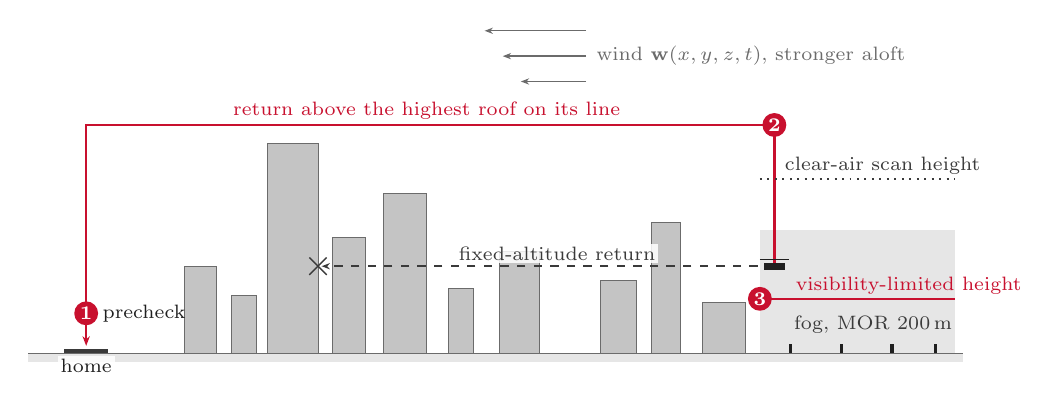
\begin{tikzpicture}[x=0.92cm,y=0.92cm,font=\scriptsize,
  bld/.style={fill=g4,draw=g2,line width=0.3pt},
  lab/.style={align=left,text=ink,font=\scriptsize,fill=white,fill opacity=0.85,text opacity=1,inner sep=1pt},
  num/.style={circle,fill=oursred,text=white,inner sep=0.8pt,font=\scriptsize\bfseries}]
  % ground
  \fill[g5] (-0.3,0) rectangle (12.6,-0.12);
  \draw[g2,line width=0.4pt] (-0.3,0) -- (12.6,0);
  % buildings
  \foreach \x/\w/\h in {1.85/0.45/1.2, 2.5/0.35/0.8, 3.0/0.7/2.9, 3.9/0.45/1.6, 4.6/0.6/2.2, 5.5/0.35/0.9,
                        6.2/0.55/1.4, 7.6/0.5/1.0, 8.3/0.4/1.8, 9.0/0.6/0.7}
    \draw[bld] (\x,0) rectangle ++(\w,\h);
  % home pad
  \fill[g1] (0.2,0) rectangle (0.8,0.06);
  \node[below=1pt,lab] at (0.5,0) {home};
  % fog layer over the scan area
  \fill[g3,opacity=0.25] (9.8,0) rectangle (12.5,1.7);
  \node[lab,fill=none,text=g1,anchor=east] at (12.5,0.4) {fog, MOR 200\,m};
  % targets
  \foreach \x in {10.2,10.9,11.6,12.2} \fill[ink] (\x,0) rectangle ++(0.05,0.12);
  % wind arrows, above everything
  \foreach \y/\l in {3.75/0.9, 4.1/1.15, 4.45/1.4}
    \draw[-{Stealth[length=3pt]},g2,line width=0.5pt] (7.4,\y) -- ++(-\l,0);
  \node[lab,fill=none,text=g2,anchor=west] at (7.5,4.1) {wind $\mathbf{w}(x,y,z,t)$, stronger aloft};
  % fixed-altitude return (crosses buildings)
  \draw[g1,dashed,line width=0.6pt,-{Stealth[length=3pt]}] (10.0,1.2) -- (3.75,1.2);
  \draw[g1,line width=0.5pt] (3.58,1.08) -- (3.82,1.32) (3.58,1.32) -- (3.82,1.08);
  \node[lab,text=g1,anchor=south] at (7.0,1.24) {fixed-altitude return};
  % geometry-aware return
  \draw[oursred,line width=0.9pt,-{Stealth[length=3.5pt]}] (10.0,1.2) -- (10.0,3.15) -- (0.5,3.15) -- (0.5,0.1);
  \node[lab,text=oursred,anchor=south] at (5.2,3.18) {return above the highest roof on its line};
  % drone
  \fill[ink] (9.85,1.15) rectangle (10.15,1.25);
  \draw[ink,line width=0.4pt] (9.8,1.29) -- (10.2,1.29);
  % scan heights
  \draw[g1,dotted,line width=0.7pt] (9.8,2.4) -- (12.5,2.4);
  \node[lab,fill=none,text=g1,anchor=south west] at (10.1,2.42) {clear-air scan height};
  \draw[oursred,line width=0.8pt] (9.8,0.75) -- (12.5,0.75);
  \node[lab,fill=none,text=oursred,anchor=south west] at (10.25,0.77) {visibility-limited height};
  % decision markers
  \node[num] at (0.5,0.55) {1};
  \node[lab,fill=none,anchor=west] at (0.68,0.55) {precheck};
  \node[num] at (10.0,3.15) {2};
  \node[num] at (9.8,0.75) {3};
\end{tikzpicture}
}
\caption{One sortie, three coupled decisions. (1) The launch precheck needs the route's energy and the wind along it.
(2) The return path must clear the buildings on the return line, and its trigger must use the same energy model as the
precheck. (3) The scan height depends on the visibility, which sets the strip spacing and the number of drones}
\label{fig:scene}
\end{figure}

\subsection{Motivational study}\label{sec:bg:study}

We quantify what goes wrong when each decision sees only part of the picture. All experiments run on the runtime of
Sect.~\ref{sec:design} with its decision-visibility switches (Sect.~\ref{sec:design:awareness}); the simulated ground
truth always stays fully coupled, and only what the decision can see changes. We use six real cities (Shenzhen,
Shanghai, Suzhou, New York, Chicago, San Francisco) built from the UrbanScene3D point clouds~\cite{lin2022urbanscene3d},
plus one procedurally generated city, and the twelve weather presets of the environment field. Energy and wind are reference models
of a 6 kg hexacopter (P600 class); we therefore report relative differences between policies rather than absolute
endurance.

\paragraph{F1: A fixed-altitude return flies into buildings.}
We draw 50,000 return starts per city on open ground, 200--1,500\,m from a home pad, and test the straight return line
at the altitude a fixed policy would fly against the city's clearance envelope: the surface model dilated by 4\,m and
raised by a 10\,m safety margin, the same envelope the runtime uses to prove a path safe. Figure~\ref{fig:m1}a shows
the share of return lines that enter the envelope for a drone loitering 40\,m above ground. With the PX4 default
(return at the higher of the current altitude and 30\,m above home, the rule of the closed-loop baseline in
Sect.~\ref{sec:eval}), 44.6\% of return lines in the six real cities enter it, from 22.6\% in San Francisco to
73.2\% in Suzhou. Raising the fixed return altitude helps but does not solve the problem: at +120\,m, 10.8\% of lines
still enter the envelope, while every return starts with a climb of about 80\,m (Fig.~\ref{fig:m1}b). A
geometry-aware return that climbs to 5\,m above the envelope's highest point on its line needs a median climb of only
2.7\,m, because most return lines are clear, but up to 612\,m when they pass a skyscraper. In none of the six cities is a
fixed altitude both safe and cheap; the right altitude is a property of each return line. The closed-loop campaigns of
Sect.~\ref{sec:eval} confirm that these envelope violations turn into physical collisions.

\begin{figure}[t]
\centering
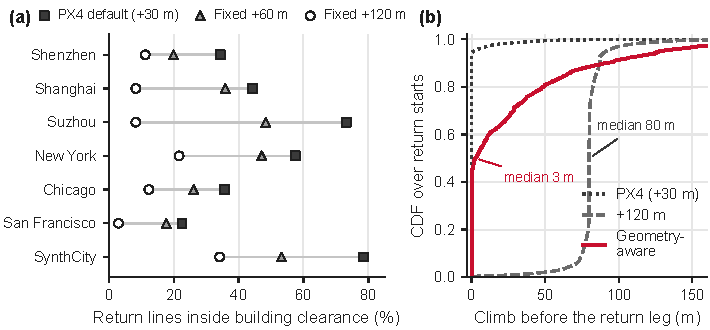
\includegraphics[width=\textwidth]{figures/pdf/m1_return_geometry.pdf}
\caption{F1, return geometry. (a) Share of straight return lines that enter the building clearance envelope for
three fixed return altitudes, drone at 40\,m above ground, 50,000 return starts per city. (b) Climb before the return leg over the six real
cities: fixed altitudes climb for every return; a geometry-aware altitude climbs only where the line requires it}
\label{fig:m1}
\end{figure}

\paragraph{F2: Wind breaks decisions through feasibility and model disagreement.}
We fly 800\,m legs on eight headings in the synthetic city under a reference-wind sweep from 0 to 16\,m/s
(Fig.~\ref{fig:m2}). Two observations stand out. First, the energy drawn per second barely changes with wind in our
reference model: below 10\,m/s the change is within $\pm$1\%, as expected on the flat bottom of the U-shaped
power curve of multirotors, where the induced power saved at higher airspeed offsets the added parasitic
power~\cite{liu2017power,bauersfeld2022range}; and a wind-blind estimate of the flown trajectory stays
within 2.5\% of the energy actually drawn (Fig.~\ref{fig:m2}b). Wind costs energy mainly through the longer
flight time against a headwind, which the shared model captures. What wind does change is \emph{feasibility}: beyond the
vehicle's 13.8\,m/s rating no leg completes. Second, and more surprisingly, wind exposes \emph{model disagreement}
between modules. When the return trigger uses its own time-based headwind model (ground speed reduced by the
headwind), as a stand-alone failsafe does, it predicts a return that the planner's energy model considers easy, and it
aborts 15--25\% of feasible legs between 2 and 12\,m/s (Fig.~\ref{fig:m2}a). When the trigger evaluates the same energy
model as the precheck, every leg below 10\,m/s completes. Wind-aware decisions thus need one shared energy and wind
model, not a better estimator in one module.

\begin{figure}[t]
\centering
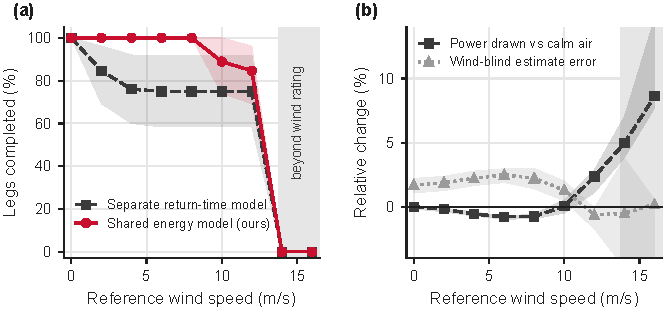
\includegraphics[width=\textwidth]{figures/pdf/m2_wind_feasibility.pdf}
\caption{F2, wind. Closed-loop 800\,m outbound and return legs, 3 seeds and 6 headings per wind speed; shaded bands are 95\%
bootstrap intervals; the shaded region on the right lies beyond the vehicle's 13.8\,m/s wind rating. (a) Legs completed when the return trigger uses a separate time-based headwind model vs the
planner's shared energy model. (b) Electrical power drawn relative to calm air, and the error of a wind-blind energy
estimate of the same trajectory}
\label{fig:m2}
\end{figure}

\paragraph{F3: A weather-blind scan plan misses targets and does not know it.}
We plan a recognition-level scan of a 500\,m area of interest at the altitude that meets the target ground sample
distance in clear air, place 400 human-sized targets on open ground, and evaluate each target's perception level with
the Johnson criteria~\cite{sjaardema2015history,vollmerhausen2004new}, using the line of sight to the camera and the
contrast attenuated by the environment field's optical depth~\cite{horvath1971koschmieder}. Figure~\ref{fig:m3}a
sweeps the meteorological optical range (MOR) for plans made for detection, recognition and identification. In clear
air about 90\% of targets reach the level; the rest are occluded by buildings. The share then collapses like a cliff,
not a slope: the recognition plan loses almost all targets between 500 and 300\,m MOR, and the detection and
identification plans, which fly at different heights, fall off between 300 and 200\,m. Across the presets
(Fig.~\ref{fig:m3}b), the weather-blind plan keeps its clear-air capture in rain, snow and thunderstorms, where
visibility stays above 0.8\,km, but the recognition plan captures 5\% of targets in fog, 0\% in a blizzard and 73\% in
a sandstorm (90\% in clear air), while predicting 99\% coverage in every case. The failure is silent: the plan is
geometrically complete, and nothing in it signals that the camera cannot see.

\begin{figure}[t]
\centering
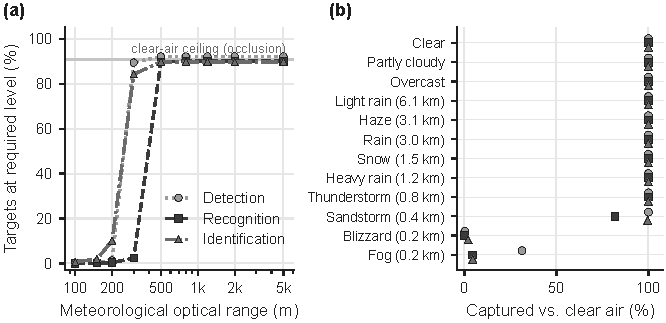
\includegraphics[width=\textwidth]{figures/pdf/m3_perception_gap.pdf}
\caption{F3, perception. (a) Targets that reach the required perception level under a scan plan made for clear air, as
the meteorological optical range (MOR) varies; 7 cities, 3 seeds per MOR. The ceiling is set by building occlusion.
(b) Capture of the same plan per weather preset relative to clear air, presets sorted by their MOR}
\label{fig:m3}
\end{figure}

\paragraph{F4: Naive coupling does not fit in the tick.}
Coupling multiplies queries: every return plan needs a corridor query along the line home, wind at the return
altitude and an energy integral, and it goes stale as the drone and the weather move. We time the naive way of keeping
every plan current, one process pinned to one core of a 64-core server (Fig.~\ref{fig:m4}). Refreshing every drone's
plan at every 4\,ms tick with an exact corridor query costs 53.8\,ms per refresh at 1,000 drones, or 13.4
core-seconds per simulated second: thirteen cores for one decision, 34 times the 0.40 core-seconds the whole pipeline
may use. Even with a sampled corridor the same schedule costs 0.15 core-seconds per simulated second, more than a third
of the pipeline budget for a single decision. Query granularity matters as much: one wind query per point costs
27.8\,$\mu$s, against 0.16\,$\mu$s per point in a batch of 10,000. Coupled decisions are therefore affordable only if
queries are batched and scheduled, not issued per drone and per tick.

\begin{figure}[t]
\centering
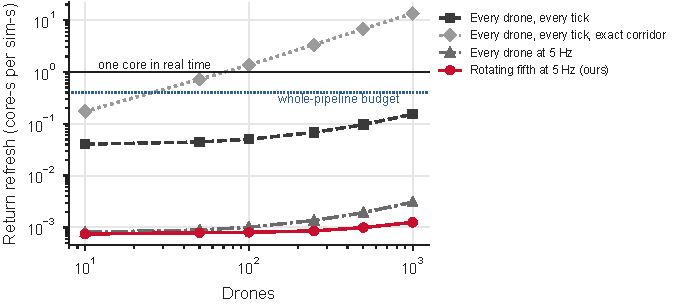
\includegraphics[width=0.86\textwidth]{figures/pdf/m4_coupling_cost.pdf}
\caption{F4, cost of coupling. CPU time to keep every drone's return plan current, per simulated second, on one core;
median of three runs. Exact corridor queries every tick exceed a full core beyond about 70 drones; the runtime's
rotating 5\,Hz schedule (Sect.~\ref{sec:design:runtime}) stays near one core-millisecond per simulated second}
\label{fig:m4}
\end{figure}


\subsection{Goals and challenges}\label{sec:bg:challenges}

The findings define three goals: decisions that see geometry, weather and energy together (F1--F3); one model shared by
the planner, the runtime and the display, so that modules do not contradict each other (F2); and coupled decisions for
a whole fleet in real time on hardware an operator actually has (F4). Reaching them raises five challenges.

\begin{description}
\item[C1 One queryable city.] City geometry arrives as point clouds, terrain models, building footprints and no-fly
zones, each with its own resolution and frame. Decisions need fast, exact answers (the highest roof along a line,
line of sight, clearance of a path) from one merged, versioned world.
\item[C2 One consistent model.] The planner, the runtime and the display must evaluate the same wind, visibility and
energy at the same place and time. Otherwise a precheck accepts what the failsafe aborts (F2) or the display shows
weather the decision did not use.
\item[C3 Perception under occlusion and weather.] Whether a target is seen depends on resolution, line of sight and
atmospheric contrast; a scan planner must work backwards from a required perception level to a flight height and
must account for visibility.
\item[C4 Real time for a fleet.] Coupled queries must fit into the 4\,ms simulation tick for 1,000 drones on a
CPU-only server.
\item[C5 Access without a server GPU.] Operators watch and steer the fleet from ordinary browsers and laptops; the
server must not render, and the client must stream a city-scale point cloud within its own budget.
\end{description}

\subsection{Related work}\label{sec:bg:related}

\paragraph{Drone simulators.} AirSim and Cosys-AirSim~\cite{shah2017airsim,jansen2023cosysairsim} render photorealistic
Unreal scenes; their wind is a single world-frame vector and their weather is a set of visual effects. Gazebo with PX4
software-in-the-loop (SITL) simulation~\cite{koenig2004gazebo,meier2015px4,furrer2016rotors} offers a uniform wind model with gusts and a linear battery
drain that feeds the failsafes. Flightmare~\cite{song2020flightmare}, gym-pybullet-drones~\cite{panerati2021learning},
RotorPy~\cite{folk2023rotorpy} and Crazyflow~\cite{schuck2026crazyflow} target control and learning; RotorPy and
Crazyflow batch more than 1,000 drones on a CPU but have no city geometry. OmniDrones~\cite{xu2024omnidrones}, Aerial
Gym~\cite{kulkarni2025aerialgym} and Pegasus~\cite{jacinto2024pegasus} build on NVIDIA Isaac
Sim~\cite{nvidia2025isaaclab,mittal2023orbit} and need a GPU. Swarm platforms such as
ARGoS~\cite{pinciroli2012argos}, SwarmLab~\cite{soria2020swarmlab}, XTDrone~\cite{xiao2020xtdrone} and the MRS
system~\cite{baca2021mrs} focus on coordination and deployment rather than on the city and the weather. CARLA, the
reference simulator for urban driving, states that weather does not affect physics~\cite{dosovitskiy2017carla}.

\paragraph{City models and aerial agents.} Embodied aerial benchmarks place agents in city scenes:
AerialVLN~\cite{liu2023aerialvln}, CityNav~\cite{lee2025citynav}, EmbodiedCity~\cite{gao2024embodiedcity} and
OpenFly~\cite{gao2025openfly}, and AerialClaw~\cite{li2026aerialclaw} drives aerial agents with language models.
Their cities are modelled for vision, and weather, energy and fleet scale are outside their scope. Urban digital
twins~\cite{batty2018digitaltwins,ketzler2020digitaltwins,shahat2021citydigitaltwin} and Web 3D formats and viewers
(3D Tiles, Potree)~\cite{ogc2023_3dtiles,schuetz2020octree,discher2019webpointclouds} stream real geometry to browsers
but do not simulate vehicles.

\paragraph{Energy, wind and return.} Multirotor power models~\cite{liu2017power,stolaroff2018energy,dorling2017vehicle,zhang2021energy}
and range estimation~\cite{bauersfeld2022range} underpin energy-aware planning; wind-aware routing for delivery
drones~\cite{ito2022wind,chakrabarty2011energy} and emergency planning under energy limits~\cite{tenharmsel2017emergency}
show that wind and energy change the best route. Studies of the urban wind
field~\cite{galway2011urban,ware2016analysis,kakavitsas2024quadrotor} and of global flyability~\cite{gao2021weather}
show how strongly the city shapes the wind and how often weather grounds drones. These works optimise one decision
under one model; we provide the shared model that lets the precheck, the return trigger and the display agree.

\paragraph{Coverage and perception.} Coverage path planning is well
surveyed~\cite{galceran2013survey,cabreira2019survey}; boustrophedon decompositions~\cite{choset2000coverage,coombes2017boustrophedon}
and energy-aware coverage~\cite{difranco2016coverage} fix the strip spacing from the camera footprint. The Johnson
criteria and the targeting task performance metric~\cite{sjaardema2015history,vollmerhausen2004new} predict the
probability of detecting, recognising and identifying a target from its resolved size and contrast, and Koschmieder's
law~\cite{horvath1971koschmieder} links contrast to visibility. We connect them: the scan planner works backwards from
the required perception level, through the visibility of the 4D field, to the flight height, strip spacing and fleet
size. Task allocation uses the contract net protocol~\cite{smith1980contract}, market-based
coordination~\cite{dias2006market,choi2009consensus} and the Hungarian method~\cite{kuhn1955hungarian}.

\paragraph{Comparison.} Table~\ref{tab:related} compares representative systems on the capabilities that coupled
urban decisions need. No existing system combines real city geometry at city scale, a weather field that drives both
the dynamics and the sensing, energy-aware decisions and 1,000-drone scale on a CPU-only server with browser access.

\begin{table}[t]
\caption{Capabilities needed for coupled urban drone decisions. \yes{} supported, \prt{} partial or only through
user-supplied assets, \no{} not supported or not documented. Evidence for every cell (documentation pages, papers) is
listed in the supplementary material.}
\label{tab:related}
\scriptsize
\setlength{\tabcolsep}{4pt}
\newcommand{\rot}[1]{\rotatebox{90}{\parbox{1.9cm}{\raggedright #1}}}
\begin{tabular*}{\textwidth}{@{\extracolsep\fill}lcccccccccc@{}}
\toprule
 & \multicolumn{2}{c}{Geometry} & \multicolumn{2}{c}{Weather} & & & \multicolumn{2}{c}{Access} & & \\
\cmidrule(lr){2-3}\cmidrule(lr){4-5}\cmidrule(lr){8-9}
System & \rot{Real city} & \rot{City scale} & \rot{Drives dynamics} & \rot{Affects sensing} & \rot{Energy-aware decisions}
 & \rot{$\geq$1,000 drones} & \rot{No server GPU} & \rot{Browser} & \rot{Deterministic replay} & \rot{Open source} \\
\midrule
AirSim/Cosys-AirSim~\cite{shah2017airsim,jansen2023cosysairsim} & \prt & \prt & \prt & \prt & \no & \no & \no & \no & \no & \yes \\
Gazebo+PX4 SITL~\cite{koenig2004gazebo,meier2015px4} & \prt & \prt & \prt & \no & \prt & \no & \prt & \prt & \prt & \yes \\
Flightmare~\cite{song2020flightmare} & \no & \no & \no & \no & \no & \prt & \prt & \no & \no & \yes \\
gym-pybullet-drones~\cite{panerati2021learning} & \no & \no & \no & \no & \no & \no & \yes & \no & \no & \yes \\
RotorPy~\cite{folk2023rotorpy} & \no & \no & \prt & \no & \no & \yes & \yes & \no & \no & \yes \\
Crazyflow~\cite{schuck2026crazyflow} & \no & \no & \no & \no & \no & \yes & \yes & \no & \no & \yes \\
OmniDrones~\cite{xu2024omnidrones} & \no & \no & \no & \no & \no & \prt & \no & \no & \no & \yes \\
Aerial Gym~\cite{kulkarni2025aerialgym} & \no & \no & \no & \no & \no & \yes & \no & \no & \no & \yes \\
Pegasus~\cite{jacinto2024pegasus} & \no & \no & \no & \no & \no & \no & \no & \no & \no & \yes \\
Isaac Sim/Lab~\cite{nvidia2025isaaclab,mittal2023orbit} & \no & \no & \no & \no & \no & \prt & \no & \prt & \no & \prt \\
MRS UAV System~\cite{baca2021mrs} & \no & \no & \no & \no & \no & \no & \no & \no & \no & \yes \\
CARLA (driving)~\cite{dosovitskiy2017carla} & \no & \prt & \no & \prt & \no & \no & \prt & \no & \yes & \yes \\
OpenFly~\cite{gao2025openfly} & \prt & \yes & \no & \no & \no & \no & \no & \no & \no & \yes \\
EmbodiedCity~\cite{gao2024embodiedcity} & \prt & \yes & \no & \no & \no & \no & \no & \prt & \no & \prt \\
CesiumJS/3D Tiles~\cite{ogc2023_3dtiles} & \yes & \yes & \no & \no & \no & \no & \yes & \yes & \no & \yes \\
Potree~\cite{schuetz2020octree} & \yes & \yes & \no & \no & \no & \no & \yes & \yes & \no & \yes \\
\midrule
\textbf{This work} & \yes & \yes & \yes & \yes & \yes & \yes & \yes & \yes & \yes & \yes \\
\botrule
\end{tabular*}
\end{table}


\section{System Design}\label{sec:design}

\subsection{Overview}\label{sec:design:overview}

Figure~\ref{fig:arch} shows the architecture of Drone4D. Three shared models sit on the left: the World Package with its geometry
query service (D1), the 4D environment field (D2), and the energy and perception models. Every consumer on the right
queries the same models through batched interfaces: the coupled decision layer (D4), the fleet runtime that produces
the simulated ground truth (D3), and the streaming access layer that feeds the operator's browser (D5). The design has
one rule that follows from F2: \emph{a quantity that two modules need is computed by one function}. The precheck and
the return trigger call the same energy model; the dynamics, the camera and the display read the same wind and optical
depth; the decision that proves a return safe and the contact stage that detects a collision read the same height map.
Table~\ref{tab:map} maps the modules to the challenges of Sect.~\ref{sec:bg:challenges}, and
Fig.~\ref{fig:matrix} lists, for each decision, which model it queries.

\begin{figure}[t]
\centering
\resizebox{\textwidth}{!}{\begingroup\newcommand{\chtagf}{\tiny\bfseries\color{oursred}}%
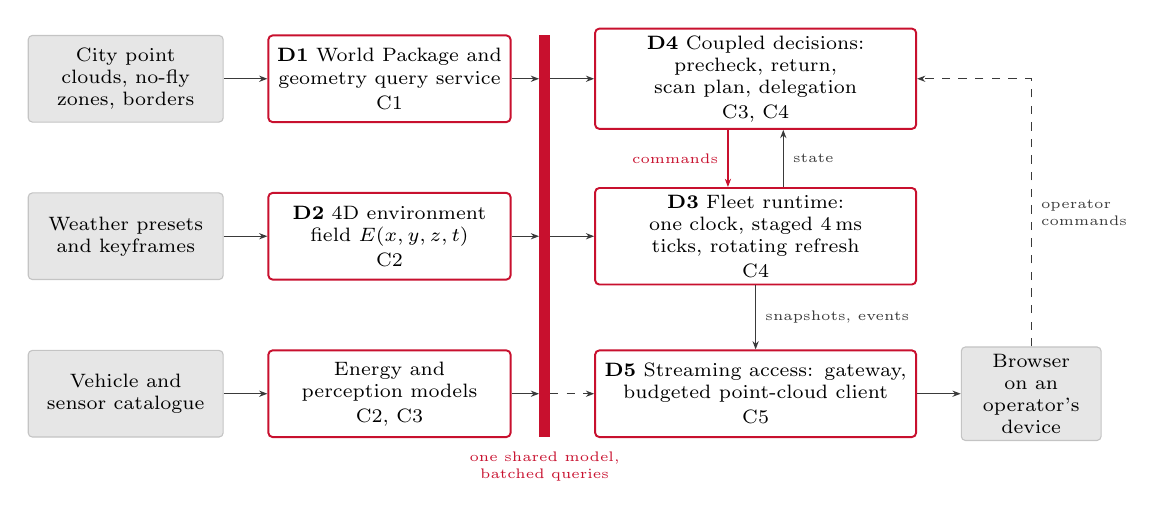
\begin{tikzpicture}[font=\scriptsize,
  box/.style={execute at begin node={\hyphenpenalty=10000},draw=g2,fill=white,rounded corners=1.5pt,line width=0.4pt,align=center,inner sep=2.5pt,
              minimum height=1.1cm},
  inp/.style={box,text width=2.3cm,fill=g5,draw=g4},
  mdl/.style={box,text width=2.9cm,draw=oursred,line width=0.7pt},
  run/.style={box,text width=3.9cm,draw=oursred,line width=0.7pt},
  arr/.style={-{Stealth[length=3pt]},g1,line width=0.45pt},
  ]
  % inputs
  \node[inp] (src) at (1.25,3.2) {City point clouds, no-fly zones, borders};
  \node[inp] (wx)  at (1.25,1.2) {Weather presets and keyframes};
  \node[inp] (veh) at (1.25,-0.8) {Vehicle and sensor catalogue};
  % shared models
  \node[mdl] (d1) at (4.6,3.2) {\textbf{D1} World Package and geometry query service\\[1pt] {\chtagf C1}};
  \node[mdl] (d2) at (4.6,1.2) {\textbf{D2} 4D environment field $E(x,y,z,t)$\\[1pt] {\chtagf C2}};
  \node[mdl] (en) at (4.6,-0.8) {Energy and perception models\\[1pt] {\chtagf C2, C3}};
  \foreach \a/\b in {src/d1, wx/d2, veh/en} \draw[arr] (\a) -- (\b);
  % bus
  \fill[oursred] (6.5,-1.35) rectangle (6.64,3.75);
  \node[font=\tiny,text=oursred,align=center,anchor=north] at (6.57,-1.42) {one shared model,\\ batched queries};
  \foreach \b in {d1,d2,en} \draw[arr] (\b.east) -- (\b.east -| 6.5,0);
  % runtime side
  \node[run] (d4) at (9.25,3.2) {\textbf{D4} Coupled decisions: precheck, return, scan plan, delegation\\[1pt] {\chtagf C3, C4}};
  \node[run] (d3) at (9.25,1.2) {\textbf{D3} Fleet runtime: one clock, staged 4\,ms ticks, rotating refresh\\[1pt] {\chtagf C4}};
  \node[run] (d5) at (9.25,-0.8) {\textbf{D5} Streaming access: gateway, budgeted point-cloud client\\[1pt] {\chtagf C5}};
  \draw[arr] (6.64,3.2) -- (d4.west);
  \draw[arr] (6.64,1.2) -- (d3.west);
  \draw[arr,dashed] (6.64,-0.8) -- (d5.west);
  % runtime internal arrows
  \draw[arr,oursred] ([xshift=-10pt]d4.south) -- node[left,font=\tiny,text=oursred] {commands} ([xshift=-10pt]d3.north);
  \draw[arr] ([xshift=10pt]d3.north) -- node[right,font=\tiny] {state} ([xshift=10pt]d4.south);
  \draw[arr] (d3.south) -- node[right,font=\tiny] {snapshots, events} (d5.north);
  % client
  \node[box,text width=1.6cm,fill=g5,draw=g4] (br) at (12.75,-0.8) {Browser on an operator's device};
  \draw[arr] (d5) -- (br);
  \draw[arr,dashed] (br.north) |- node[pos=0.25,right,font=\tiny,text=g1,align=left] {operator\\commands} (d4.east);
\end{tikzpicture}\endgroup
}
\caption{Architecture. Shared models (left) are queried in batches on the simulation clock by the decision layer and
the fleet runtime (solid) and streamed to the browser (dashed). The tags C1--C5 give the challenge each module addresses}
\label{fig:arch}
\end{figure}

\begin{table}[t]
\caption{Design modules, the challenges they address and the mechanisms that address them.}
\label{tab:map}
\footnotesize
\begin{tabular*}{\textwidth}{@{\extracolsep\fill}llp{6.3cm}@{}}
\toprule
Module & Challenge & Key mechanism \\
\midrule
D1 World Package, geometry service & C1 & Versioned package, max-pyramids, exact and bounded corridor queries \\
D2 4D environment field & C2 & One analytic field for wind, visibility and optics; golden vectors for every client \\
D3 Fleet runtime & C4 & One 250\,Hz clock, staged sub-rates, structure-of-arrays kernels, rotating return refresh \\
D4 Coupled decision layer & C3, C4 & Shared-energy return trigger, wind-rated precheck, level-driven scan planner \\
D5 Streaming access & C5 & Headless server, budgeted point-cloud selection with a cascade controller \\
\botrule
\end{tabular*}
\end{table}

\begin{figure}[t]
\centering
\begingroup
\newcommand{\cellq}[2]{\node[circle,fill=oursred,inner sep=1.5pt] at (#1) {};
  \node[font=\tiny,text=ink,align=center,anchor=north,text width=1.7cm,
        execute at begin node={\hyphenpenalty=10000}] at ($(#1)+(0,-0.12)$) {#2};}
\newcommand{\celln}[1]{\node[circle,draw=g3,inner sep=1.4pt] at (#1) {};}
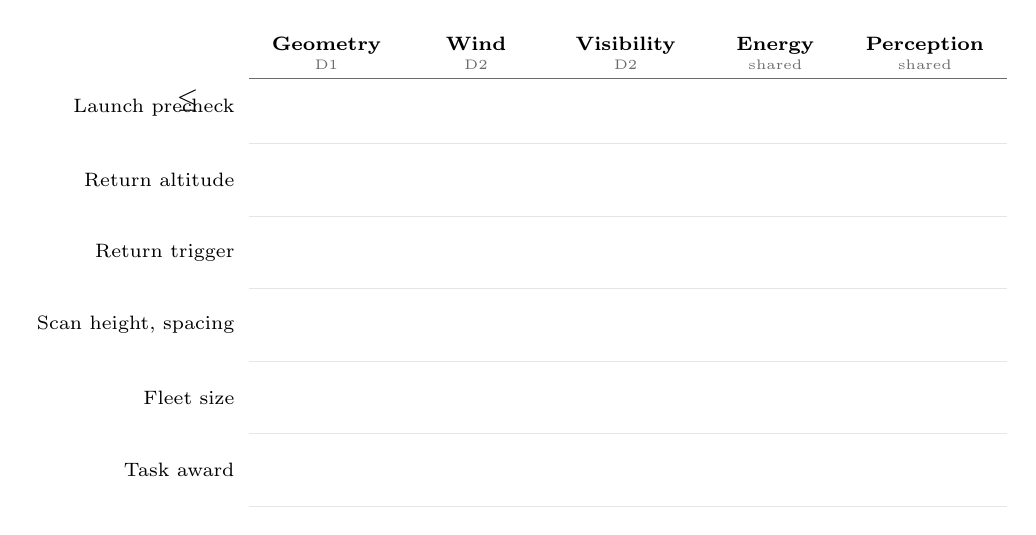
\begin{tikzpicture}[font=\scriptsize,x=1.9cm,y=0.92cm]
  % header
  \foreach \c/\t/\d in {1/Geometry/D1, 2/Wind/D2, 3/Visibility/D2, 4/Energy/shared, 5/Perception/shared}
    \node[font=\scriptsize\bfseries,align=center] at (\c,0.75) {\t\\[-1pt]{\tiny\mdseries\color{g2}\d}};
  % rows
  \foreach \r/\t in {0/Launch precheck, 1/Return altitude, 2/Return trigger, 3/{Scan height, spacing},
                     4/Fleet size, 5/Task award}
    {\node[anchor=east,align=right,font=\scriptsize] at (0.45,-\r) {\t};
     \draw[g5,line width=0.4pt] (0.48,-\r-0.5) -- (5.55,-\r-0.5);}
  \draw[g2,line width=0.5pt] (0.48,0.4) -- (5.55,0.4);
  % row 0: precheck
  \cellq{1,0}{cruise above the route's roofs}
  \cellq{2,0}{route wind vs rating}
  \celln{3,0}
  \cellq{4,0}{out + station + return $\le$ reserve}
  \celln{5,0}
  % row 1: return altitude
  \cellq{1,-1}{highest roof on the line, detour}
  \cellq{2,-1}{headwind of candidates}
  \celln{3,-1}
  \cellq{4,-1}{climb vs detour energy}
  \celln{5,-1}
  % row 2: return trigger
  \cellq{1,-2}{climb to return altitude}
  \cellq{2,-2}{wind at return altitude}
  \celln{3,-2}
  \cellq{4,-2}{same model as precheck}
  \celln{5,-2}
  % row 3: scan
  \cellq{1,-3}{obstacle cells, line of sight}
  \celln{2,-3}
  \cellq{3,-3}{optical depth caps height}
  \celln{4,-3}
  \cellq{5,-3}{pixels for D/R/I}
  % row 4: fleet size
  \celln{1,-4}
  \cellq{2,-4}{sortie endurance in wind}
  \cellq{3,-4}{lower height, more strips}
  \cellq{4,-4}{per-sortie energy}
  \celln{5,-4}
  % row 5: award
  \cellq{1,-5}{line of sight to the task}
  \cellq{2,-5}{weather risk term}
  \cellq{3,-5}{expected detection}
  \cellq{4,-5}{precheck of the bid}
  \cellq{5,-5}{sensor capability}
\end{tikzpicture}
\endgroup

\caption{Decision-coupling matrix. A filled dot means the decision queries that model, with the query it makes; an
open dot means it does not. Every filled dot in a column is the same function call}
\label{fig:matrix}
\end{figure}

\subsection{World Package and geometry query service}\label{sec:design:world}

\paragraph{Package.} A city enters the system as a point cloud plus semantic layers (borders, no-fly zones). An
offline pipeline normalises units, axes and origin, derives a 10\,m terrain model by morphological opening, classifies
points by height above ground, tiles the visual cloud into an octree with a 12-byte quantised point encoding, and
derives a 2\,m digital surface model (DSM). The result is published atomically as a World Package whose content version is
the hash of its files. Six real cities from UrbanScene3D~\cite{lin2022urbanscene3d} and one procedural city are
built this way; a city occupies 138--192\,MB.

\paragraph{Derived geometry.} At load time the service derives, and caches under a key that combines the content
version with the derivation parameters, a clearance height map $H = \mathrm{maxfilter}_{5\times5}(\mathrm{DSM}) + 10$\,m,
max-pooled pyramids of the surface and of the height map, a dilated height-map pyramid for corridor queries, and an
8\,m raster of no-fly zones. Because $H$ is dilated and raised, a path that clears $H$ also clears the inflated
surface model; this monotonicity lets cheap coarse checks certify a path against the model and leaves fine checks for the few paths that need
them.

\paragraph{Queries.} Decisions use a small set of vectorised queries: surface and terrain height, the maximum of $H$
along a segment (exact cell traversal or a bounded pyramid sample with a 100\,m tolerance), batched line of sight (up
to 64 pairs per call), coarse path checks that classify each segment as proven safe, uncertain or violating against
both $H$ and the zones, fine path validation at 20 samples per metre, and a safe-transit profile that climbs to
$\max_{\text{line}} H + 5$\,m. The same height map drives the return altitude in D4 and the contact stage in D3, so
the decision and the ground truth cannot disagree about what a building is.

\subsection{4D environment field}\label{sec:design:env}

\paragraph{One analytic field.} The environment is a function $E(x,y,z,t)$ evaluated on demand rather than a stored
grid. Wind is composed as
\begin{equation}
\mathbf{w}(x,y,z,t) = s(t)\, f\big(z_{\mathrm{agl}}\big)\, \mathbf{e}(\theta(t)) + \textstyle\sum_k \mathbf{G}_k(x,y,z,t)
 + g(z)\,\mathbf{T}(x,y,z,t),
\end{equation}
a reference speed $s$ and direction $\theta$ shaped by a logarithmic profile
$f(z) = \ln\!\big((z-d)/z_0\big)/\ln\!\big((z_{\mathrm{ref}}-d)/z_0\big)$ with the city's roughness length $z_0$ and
displacement height $d$, plus discrete gusts $\mathbf{G}_k$ and turbulence $\mathbf{T}$ from a periodic $64^3$ box and a
Dryden filter bank~\cite{beal1993digital}; height above ground comes from the World Package's terrain model. The
atmosphere carries the meteorological optical range, the extinction coefficient, precipitation and fog-top height, and
the standard-atmosphere state. Slant optical depth $\tau(\mathbf{p}_0,\mathbf{p}_1,t)$ integrates an exponential haze
profile, a fog slab and precipitation below the cloud base, and gives the transmittance $e^{-\tau}$ that perception uses.
Twelve presets (clear to blizzard and sandstorm) set 21 scalar parameters; changes are applied as keyframes of at most
2\,KB that interpolate over time, so a weather change is a few bytes on the wire.

\paragraph{One field for every consumer.} The field is queried in batches of up to 256 points with a time argument.
The fleet runtime evaluates it at 50\,Hz for every drone and writes wind and air density into the dynamics; the
camera model evaluates optical depth per target; the decision layer evaluates it along candidate routes; and the
browser evaluates the same equations in TypeScript for the display. A shared set of golden vectors (profiles, gusts,
turbulence, keyframe evaluation, optical depth) is checked by both the Python and the TypeScript test suites, so the
display evaluates the same field the drones fly in (Sect.~\ref{sec:eval:consistency}); how faithfully the rendered
effects convey that field to an operator is a separate question we do not study here.

\subsection{Fleet runtime on one clock}\label{sec:design:runtime}

\paragraph{One clock, staged sub-rates.} All drones share one 250\,Hz simulation clock (4\,ms ticks). Work is split
into stages that each declare a period in ticks and a phase: the environment and sensors run at 50\,Hz, the
dynamics and contact at 125\,Hz, inter-drone collision at 25\,Hz, energy integration at 10\,Hz and return-plan refresh
at 5\,Hz. Phases are staggered to spread the expensive stages over different ticks. Every stage declares a CPU budget in
core-seconds per simulated second; the runtime refuses to build a pipeline whose budgets sum to more than 0.40 at
1,000 drones and real time, and it reports the measured cost of each stage once per second.

\paragraph{Structure of arrays.} The state of up to 1,024 drones lives in contiguous arrays (position, velocity,
attitude, battery, safety state), and every stage is a vectorised kernel over all drones or over a subset. The flight
controller is a PX4-like cascaded position and attitude controller; the power drawn is
$P = P_{h}\,(T/T_{h})^{1.5}$ plus a climb term, evaluated with the airspeed implied by the local wind. Contact against
the surface model, inter-drone separation with hold and resume, a flight state machine (flying, hold, return with
climb, cruise, descend and final phases, landing, emergency landing) and seeded random streams complete the ground
truth. No stage reads the wall clock, so a run is a deterministic function of its seed and its command log, and the
recorder can replay it.

\paragraph{Rotating refresh.} Return plans are the most expensive per-drone decision: each needs a corridor query
along the line home, a wind query at the return altitude and an energy integral. Instead of refreshing every drone on
every call, the 5\,Hz return stage refreshes a rotating fifth of the fleet, so each plan is at most one second old. Section~\ref{sec:eval:micro}
measures what this buys.

\subsection{Coupled decision layer}\label{sec:design:decisions}

\subsubsection{Decision awareness}\label{sec:design:awareness}

Each decision reads the shared models through a switchboard, \texttt{DecisionAwareness}, with one flag per factor:
\texttt{geometry} (corridor height map), \texttt{detour} (detour candidates), \texttt{wind} (field wind instead of
calm air), \texttt{visibility} and \texttt{los} (optical depth and line of sight in the detector quote),
\texttt{energy\_rtl} (energy-based return trigger), \texttt{precheck\_env} (field wind in the precheck) and
\texttt{shared\_energy} (return trigger on the precheck's energy model). A fixed-altitude policy reproduces the PX4
default. The flags change only what a decision \emph{sees}; the simulated ground truth is always fully coupled. This
makes every baseline and ablation of Sect.~\ref{sec:eval} a configuration of one system rather than a different
code base.

\subsubsection{Launch precheck}

Before a sortie the precheck builds the route the planner will fly, take-off, a climb to the cruise altitude
$z_c = \max(z_{\mathrm{op}}, z_{\mathrm{pad}} + 25, \max_{\text{route}} H + 5)$, the transit, the station time and the
return, and integrates the shared energy model along it with the field wind. A sortie launches only if
\begin{equation}
\mathrm{soc}_0 - \frac{E_{\mathrm{out}} + E_{\mathrm{station}} + E_{\mathrm{back}}}{E_{\mathrm{use}}} \geq r
\quad\text{and}\quad \max_{\text{route}} \lVert \mathbf{w}_{xy} \rVert \leq w_{\mathrm{rating}},
\end{equation}
with usable energy $E_{\mathrm{use}}$, reserve $r = 0.20$ and the vehicle's wind rating $w_{\mathrm{rating}}$
(13.8\,m/s for the P600 profile). The second condition encodes F2: wind matters mainly through feasibility.

\paragraph{Space-time precheck.} The environment field's keyframe defines the weather for the whole of its transition,
so a forecast front is part of the shared model. The space-time variant evaluates each leg at the time it will be
flown: the transit at launch time, the station and the return at their predicted start times $t_{\mathrm{back}} =
t_{\mathrm{out}} + t_{\mathrm{station}}$, with wind sampled along each leg over its duration. If the requested station
time would put the return into wind beyond the rating or below the reserve, the precheck shortens the station time in
15\,s steps, down to 30\,s, and declines the sortie only if even that fails. It costs one batched field query per
candidate station time.

\subsubsection{Return planning}

\paragraph{Altitude and path.} The return altitude is
$z_{\mathrm{rtl}} = \max\big(z_{\mathrm{now}},\, z_{\mathrm{home}} + 30,\, \max_{[\mathbf{p},\mathbf{h}]} H + 5\big)$:
the PX4 rule plus the corridor term that F1 shows to be necessary. When the corridor term forces a climb of more than
10\,m, the planner evaluates single-waypoint detours $\mathbf{p} + fL\mathbf{u} + kw\mathbf{n}$ to either side of the
line, each with its own corridor height and headwind, and keeps the one that shortens the return by at least 5\,s; at
most 16 drones run the detour search per refresh to bound its cost.

\paragraph{Trigger on the shared energy model.} The return starts when the remaining flight time falls below
$1.3\,t_{\mathrm{rtl}}$ or the state of charge below 7\%. A stand-alone failsafe estimates $t_{\mathrm{rtl}}$ from
distances and a cruise speed reduced by the headwind, which is the model disagreement of F2. With
\texttt{shared\_energy}, $t_{\mathrm{rtl}}$ is instead the energy-equivalent time of the planned return under the same
model the precheck uses:
\begin{equation}
t_{\mathrm{rtl}} = \frac{E_{\mathrm{climb}} + E_{\mathrm{cruise}}(\mathbf{w}) + E_{\mathrm{descent}}}{\max(\bar P,\, 0.5\,P_h)},
\end{equation}
where the cruise term integrates the power at the airspeed implied by the field wind at $z_{\mathrm{rtl}}$, the ground
speed is held unless the headwind exceeds the wind rating, and $\bar P$ is the current average power. Both decisions
now ask the same question of the same function, so the trigger fires when the energy, not a second model, runs out.

\subsubsection{Perception-driven scan planning}

\paragraph{From level to pixels.} For a target with projected critical dimension $d_c = \sqrt{A_{\mathrm{proj}}}$
seen at range $R$ through a lens of focal length $f$ on pixels of pitch $p$, the number of pixels on target is
$N = d_c f/(R\,p)$. The targeting task performance function~\cite{vollmerhausen2004new} gives the probability of a task
as $P(N) = x^{E}/(1+x^{E})$ with $x = N/(2N_{50})$ and $E = 2.7 + 0.7x$, where the Johnson cycle criteria
$N_{50} = 1, 4, 6.4$ correspond to detection, recognition and identification~\cite{sjaardema2015history}. At
$P = 0.9$ this requires 3.5, 14.0 and 22.4 pixels. Atmospheric contrast $C = C_0\,e^{-\tau(R)}$, with $\tau$ from D2,
scales the usable resolution by $k_c = \mathrm{clip}\big((C - 0.05)/(0.25 - 0.05), 0, 1\big)$, and a blocked line of
sight sets it to zero.

\paragraph{From pixels to a fleet.} For each candidate flying height $H$ above ground the planner (i) drops the cells
whose buildings rise above $H$ minus the clearance and rejects $H$ if they exceed 5\% of the area, (ii) computes the
slant range at the strip edge $R_e = H/\cos\theta_e$ ($\theta_e \leq 15^{\circ}$) and the focal length
$f \geq N_{\mathrm{req}} R_e\, p/(d_c\, k_c)$ needed there under the current optical depth, rejecting $H$ if no lens
reaches it, (iii) derives the ground sample distance, the strip width $w = \min(W g,\, 2H\tan\theta_{\max})$ and the
spacing $(1-s)w$, and (iv) lays out boustrophedon strips~\cite{choset2000coverage} at the best sweep angle. It keeps the
height with the shortest single-drone time, then picks the smallest number of drones whose balanced partition, assigned
to depots with the Hungarian method~\cite{kuhn1955hungarian}, fits a sortie budget
$T_{\max} = \min\big(t_{\mathrm{cap}},\, 0.8\,t_{\mathrm{sortie}}(\mathbf{w}) - 2\,t_{\mathrm{transit}}\big)$, where the
sortie endurance comes from the shared energy model under the current wind. Visibility therefore propagates through the
whole plan: lower visibility lowers the height, narrows the strips, lengthens the plan and raises the number of drones,
and the planner reports this cost instead of silently losing targets (F3).

\subsubsection{Capability-based task delegation}

Tasks that need a specific sensor are delegated with the contract net protocol~\cite{smith1980contract}: the
coordinator announces the task to the drones whose capability matches, each drone returns a quote, and the task is
awarded to the best score
$U = w_c\,\hat c - w_t\,\eta/\eta_0 - w_e\,E/E_0 - w_l\,\ell - w_r\,\rho$,
where the expected confidence $\hat c$ comes from the detector quote with optical depth and line of sight, $\eta$ and
$E$ come from the same precheck as a launch, $\ell$ is the drone's load and $\rho$ a weather-risk term from the field.
Infeasible quotes score $-\infty$.

\subsection{Streaming access without a server GPU}\label{sec:design:access}

The server runs the simulation headless on CPUs and never renders. A gateway publishes compact per-drone state at up
to 125\,Hz of simulation time (clients typically subscribe at 10--20\,Hz), events, keyframes of the environment field
and a 10\,Hz time message, with credit-based back-pressure, and it reports the age of the data it serves. The browser
renders the city point cloud with WebGL2 from HTTP range requests on the octree tiles and evaluates the environment
field locally for weather effects. Its point budget is chosen by two controllers. APH (adaptive prefix with hysteresis)
selects octree nodes best-first by screen-space error under a point budget $B$, always keeps the nodes required for a
coherent view, and applies hysteresis to avoid popping. CAS (a cascade controller) adapts $B$: an inner loop adjusts
$B$ in the log domain every 250\,ms from a 24-frame window against a 33.3\,ms frame target, and an outer loop moves
between seven quality rungs. The client therefore holds its frame rate on a laptop GPU or a software renderer,
without any GPU on the server (Sect.~\ref{sec:eval:access}).

\section{Evaluation}\label{sec:eval}

We ask four research questions. 
(1) Do coupled decisions make urban sorties safer and more productive than the decoupled practice
of today (Sect.~\ref{sec:eval:overall})? 
(2) Which coupling is responsible for which part of the gain (Sect.~\ref{sec:eval:ablation})? 
(3) What does the coupling cost, and does the runtime keep it inside the real-time budget
of a fleet (Sect.~\ref{sec:eval:micro})? 
(4) Can operators reach the runtime from ordinary devices without a server GPU (Sect.~\ref{sec:eval:access})? 
We then test how sensitive the results are to the decision parameters
(Sect.~\ref{sec:eval:sens}) and whether the shared model is in fact the same model everywhere
(Sect.~\ref{sec:eval:consistency}).

\subsection{Setup}\label{sec:eval:setup}

Table~\ref{tab:config} summarises the configuration. All campaigns run the complete runtime of Sect.~\ref{sec:design}
in-process with a simulated clock that advances faster than real time; only the decision-awareness switches differ
between policies, and the simulated ground truth (wind acting on the dynamics, contact with the surface model, battery
discharge) is always fully coupled. A sortie is \emph{completed} if the drone lands within 25\,m of its depot,
\emph{lost} if it collides with a building or the ground or ends away from home with an empty battery, \emph{returned
early} if the battery logic recalls it before its station time ends, and \emph{not launched} if the precheck refuses
it. We call a sortie \emph{unsafe} if it is lost or if it is launched although the field wind along its route exceeds
the vehicle's 13.8\,m/s rating. Intervals are 95\% percentile bootstrap intervals; for closed-loop campaigns the bootstrap resamples whole
tasks (city, weather and seed), because the sorties of one task share their conditions. Large language models were used
to help search the literature and edit the text and to produce simulated reviewer critiques of a draft; they did not
generate, select or analyse any experimental data.

\begin{table}[t]
\caption{Experiment configuration.}\label{tab:config}
\footnotesize
\begin{tabularx}{\textwidth}{@{}lX@{}}
\toprule
Server & 64-core Intel Xeon Gold 6426Y, 503\,GB RAM, Linux 6.8, Python 3.12; no GPU used by the runtime \\
Clients & Apple M3 laptop (Chrome, Metal); headless Chromium on the server with SwiftShader (software) and with an NVIDIA A100 (Vulkan) \\
Cities & Shenzhen, Shanghai, Suzhou, New York, Chicago, San Francisco (UrbanScene3D~\cite{lin2022urbanscene3d}) and SynthCity (procedural, 1.2\,km) \\
Weather & the 12 presets of the environment field, from clear to thunderstorm; wind direction drawn per seed \\
Vehicle & P600-class hexacopter reference model: 222\,Wh battery, 85\% usable, 20\% launch reserve, wind rating 13.8\,m/s \\
Return campaign & 8 drones per task, on-station points at 40\,m above ground 300--1,100\,m from the depot, station time 30--300\,s, \RTLSEEDS{} seeds per city and preset, 9 policies (\RTLSORTIES{} sorties) \\
Scan campaign & 500\,m area of interest, 400 standing persons on open ground, detection, recognition and identification plans, 3 seeds per city and preset, plus a MOR sweep from 100\,m to 5\,km \\
Front campaign & sorties as above launched in clear air while the weather turns into rain, heavy rain or a thunderstorm over 10\,min; 5 seeds per city and front; PX4 default, snapshot and space-time precheck \\
Delegation & 12 drones (half with a 4.8--48\,mm zoom, half with a fixed 4.8\,mm lens), state of charge 12--90\%, 30 observation requests per task, 5 seeds per city and preset \\
Policies & PX4 default return (climb to 30\,m above home, straight line, battery thresholds) without mission precheck; a decoupled stack (wind-blind energy precheck, geometry- and wind-blind return); the coupled policy; and one ablation per coupling. Scan: weather-blind plan sized for clear air vs coupled plan. Delegation: nearest drone, contract net with clear-air perception quotes, and coupled contract net \\
\bottomrule
\end{tabularx}
\end{table}

\subsection{Overall performance}\label{sec:eval:overall}

\paragraph{Launch and return.} Figure~\ref{fig:overall-heatmap} shows, for every city and weather preset, the share of
sorties that end unsafe under the PX4 default and under the coupled policy, and the share the coupled policy completes.
Under the PX4 default, \PXUNSAFE\% of all sorties are unsafe: in calm and wet weather most of them are returns that fly
into buildings, between \PXCITYLO\% of sorties in \PXCITYLOW{} and \PXCITYHI\% in \PXCITYHIW{}, and in severe weather every launched
sortie flies beyond the wind rating. The coupled policy reduces the unsafe share to \CPUNSAFE\% and at the same time
completes \CPDONE\% of sorties instead of \PXDONE\%. Of its 34 residual collisions, 30 occur on one pad of the San
Francisco depot, within one metre of the pad at lift-off or touchdown, and the same sorties collide under the other
policies as well; they are a property of that pad cell in the surface model rather than of a decision. The other four
are collisions between two returning drones in SynthCity, which the separation layer, not the return planner, has to
resolve. The decoupled stack, which adds a wind-blind energy precheck to a geometry-
and wind-blind return, behaves like the PX4 default (\DCUNSAFE\% unsafe, \DCDONE\% completed): an energy precheck
alone does not help when the return it budgets for is the wrong one.

\begin{figure}[t]
\centering
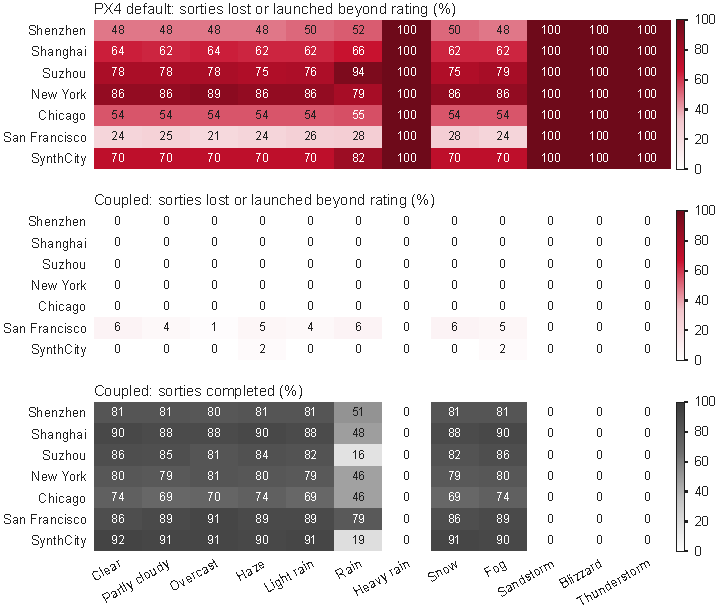
\includegraphics[width=\textwidth]{figures/pdf/overall_heatmap.pdf}
\caption{Overall performance per city and weather preset (\RTLSEEDS{} seeds, 8 sorties each). Top: sorties lost or
launched beyond the wind rating under the PX4 default. Middle: the same under the coupled policy. Bottom: sorties the
coupled policy completes. Presets in which the field wind exceeds the rating are not launched by the coupled policy}
\label{fig:overall-heatmap}
\end{figure}

Figure~\ref{fig:overall-outcomes}a breaks the outcomes down by weather group. In calm weather the coupled policy
completes \CPCALMDONE\% of sorties against \PXCALMDONE\% for the PX4 default, because the PX4 default loses \PXCALMLOST\% of its sorties on the
way home; the coupled policy declines \CPCALMDECL\% of the calm-weather sorties, whose cruise altitude over the
buildings is about twice that of the launched ones and whose mission energy would break the launch reserve. In wet and windy weather the coupled policy declines \CPWETDECL\% of the sorties, those whose route wind
exceeds the rating or whose return under the field wind would break the reserve, and completes \CPWETDONE\%; the PX4 default
launches all of them, completes \PXWETDONE\% and flies \PXWETOVER\% beyond the rating. In severe weather the coupled policy launches
nothing, while the PX4 default loses \PXSEVLOST\% of its sorties. Declining is the honest answer in these cases, and the
precheck reports it before take-off instead of discovering it in flight.

Where does the safety come from? Figure~\ref{fig:overall-outcomes}b shows how high the returns climb above the depot.
The PX4 default returns at the higher of its current altitude and 30\,m above home, so a drone on station 40\,m above
the ground flies home at about its station altitude (median \PXCLIMB\,m above the depot), and collides on
\PXCOLL\% of sorties. Climbing over the highest point of the clearance envelope on the return line removes the collisions
but makes the median return climb \NDCLIMB\,m. The coupled policy keeps the same collision rate with a median climb of
\CPCLIMB\,m, because detours around tall buildings replace the largest climbs, and spends \CPRETWH\,Wh per return against
\NDRETWH\,Wh.

\begin{figure}[t]
\centering
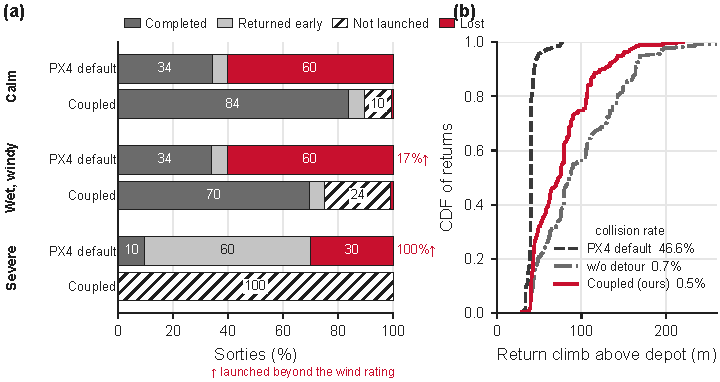
\includegraphics[width=\textwidth]{figures/pdf/overall_outcomes.pdf}
\caption{Outcome of every sortie. (a) Outcome shares per weather group; numbers with an upward arrow to the right are the sorties
launched beyond the wind rating. (b) Distribution of the return climb above the depot, with each policy's collision
rate over all sorties}
\label{fig:overall-outcomes}
\end{figure}

\paragraph{Weather fronts.} The campaigns above hold the weather constant. To test the time dimension of the shared
model, we launch the same sorties in clear air while the field holds a front that turns the weather into rain, heavy
rain or a thunderstorm over the next 10 minutes (7 cities, 5 seeds, 840 sorties per policy and front). Because the
transition is part of the field's keyframe, the space-time precheck of Sect.~\ref{sec:design:decisions} can query it
at the times the legs will be flown, while the snapshot precheck of the coupled policy sees only the clear air at
launch. We record the largest field wind at each drone's position during the flight and call a sortie unsafe if it is
lost or meets wind beyond the rating (Fig.~\ref{fig:front}). The snapshot precheck launches nearly every sortie into
the front: 40\%, 85\% and 89\% of its sorties are unsafe, and in the thunderstorm it loses 49\% of its sorties, 104 of the 137 lost in
emergency landings away from home once the drone can no longer hold its position. The PX4 default is worse still (65\%,
94\%, 96\%). The space-time precheck reduces the unsafe share to 11\%, 8\% and 4\%: it shortens the station time of
60--76\% of the sorties it launches into heavy rain and thunderstorms, to about two thirds of the request, and declines
those that cannot be back before the front. It delivers more safe station time than either alternative in heavy rain
and thunderstorms, and 11 points less than the snapshot precheck in rain, where its route wind, sampled at the cruise
altitude, is conservative. The precheck samples the route wind at three points of each leg; its remaining unsafe
sorties met stronger wind elsewhere on the path they actually flew.

\begin{figure}[t]
\centering
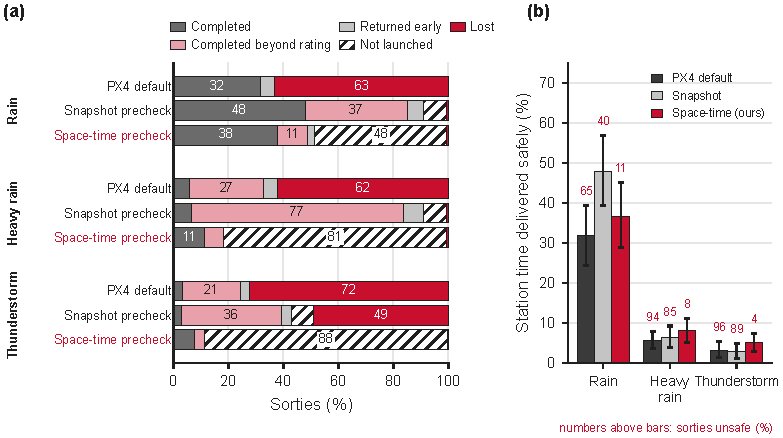
\includegraphics[width=\textwidth]{figures/pdf/front.pdf}
\caption{Weather fronts: sorties launched in clear air while a front builds over 10 minutes. (a) Outcome of every
sortie; ``completed beyond rating'' sorties came home but met field wind beyond the 13.8\,m/s rating. (b) Station
time delivered by sorties that came home within the rating, as a share of the requested station time; the numbers above the bars
are the unsafe sorties (lost or beyond the rating). Bars show 95\% task-level bootstrap intervals}
\label{fig:front}
\end{figure}

\paragraph{Scan planning.} Figure~\ref{fig:coverage-eval} evaluates the perception-driven scan planner of
Sect.~\ref{sec:design:decisions} in the three presets that reduce visibility. A weather-blind plan sized for clear air
captures 34\% of targets at detection level in fog and 5\% at recognition and identification level, and almost none in
a blizzard. The coupled planner flies lower and narrower strips under the field's optical depth and captures 82--91\%,
within a few points of the clear-air ceiling set by building occlusion. In a sandstorm, where visibility is reduced
less, the blind plan only loses recognition capture (73\% vs 89\%). The coupled plan reports the price of this capture
before launch: 1.34--1.41 times as many drones for recognition and identification and 1.05--1.27 times the makespan
(Fig.~\ref{fig:coverage-eval}b). In every other preset the two plans coincide, so the coupling costs nothing when the
weather does not matter. Planners that see only one of the two inputs separate their roles: a plan that knows the
visibility but not the wind captures as much as the coupled plan, while a plan that knows only the wind captures as
little as the blind one. Wind instead decides whether the sorties fit the battery: the endurance under the field wind is
6\% shorter than the blind plan's sortie budget on average and up to 29\% shorter, while the coupled budget matches
it. Capture is scored on the planned trajectories with the perception model; flying the scans in closed loop
is left to future work.

\begin{figure}[t]
\centering
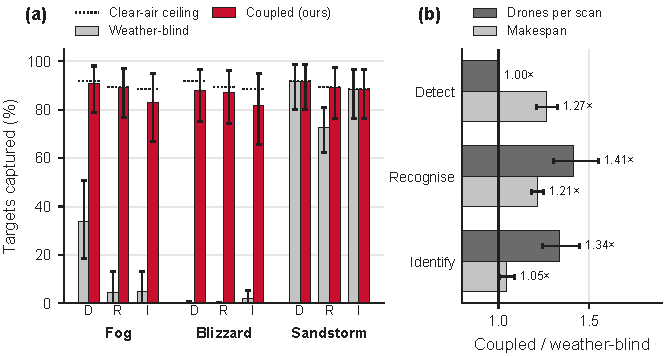
\includegraphics[width=\textwidth]{figures/pdf/coverage_eval.pdf}
\caption{Scan planning in low visibility, 7 cities and 3 seeds per preset. (a) Targets captured at the required level
(D detection, R recognition, I identification) by the weather-blind and the coupled plan; dotted lines are the
clear-air capture of the same tasks. (b) Drones per scan and makespan of the coupled plan relative to the blind plan,
over the feasible plans in the three presets}
\label{fig:coverage-eval}
\end{figure}

\paragraph{Task delegation.} Observation requests (a standing person to be detected, recognised or identified) are
delegated to a heterogeneous fleet: half the drones carry a zoom camera and half a fixed wide lens, and their states of
charge range from 12\% to 90\%, as between sorties. Every candidate quotes a request against the shared models: the
energy of the flight out at a corridor-safe altitude, a 60\,s observation and the flight home under the field wind,
and the perception level reached from the best of eight viewpoints around the target, with line of sight and slant
optical depth. Figure~\ref{fig:delegation} compares three awards on the same requests. Awarding the nearest drone, as
a distance-only dispatcher does, completes 42.2\% of requests. Of all its awards (one per request), 34.1\% break the launch reserve, among them
16.2\% that would strand the drone, and 35.8\% send a drone beyond the wind rating (the two overlap in strong wind); and a wide-lens drone is often nearest when a zoom
is needed. A contract net whose perception quote ignores line of sight and the atmosphere never breaks the reserve but
completes only 47.3\%, because it picks drones that cannot resolve the target. The contract net on the shared models
completes 58.6\% of requests, 94.2\% in clear air, never breaks the reserve, and declines the 37.8\% that no drone can
serve safely, mostly in thunderstorms, blizzards and sandstorms. The price is a 10\% longer time to the target (106\,s
against 96\,s), because the best drone is not always the nearest.

\begin{figure}[t]
\centering
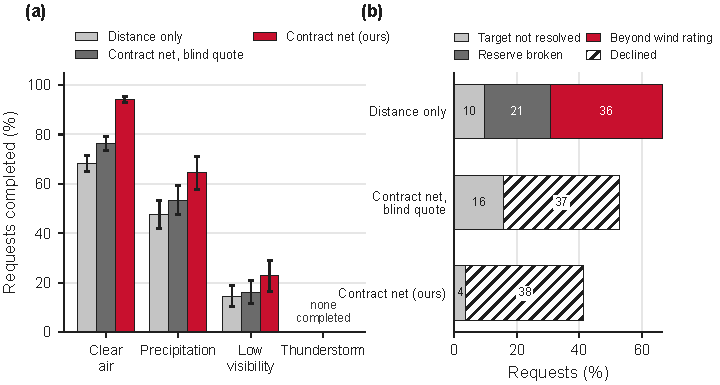
\includegraphics[width=\textwidth]{figures/pdf/delegation.pdf}
\caption{Capability-based delegation, 7 cities, 12 presets, 5 seeds, 30 requests each (12,600 requests per policy).
(a) Requests completed per weather group. (b) Why requests fail: the awarded drone cannot resolve the target, the
flight breaks the launch reserve, the route exceeds the wind rating, or the request is declined because no drone can
serve it}
\label{fig:delegation}
\end{figure}


\subsection{Ablation}\label{sec:eval:ablation}

Figure~\ref{fig:ablation} removes one coupling at a time from the coupled policy, on the same sorties. Each variant
turns off one decision-visibility switch of Sect.~\ref{sec:design:awareness} (\texttt{geometry}, \texttt{detour},
\texttt{wind}, \texttt{shared\_energy}, \texttt{energy\_rtl}) or the precheck; ``w/o detour'' is the
climb-to-clear return, which flies over the highest point of the envelope on the return line.
\begin{itemize}
\item \textbf{Geometry} is responsible for the safety of the return: without the corridor term, \NGCOLL\% of sorties
collide, and the share completed falls from \CPDONE\% to \NGDONE\%. The energy per completed sortie drops, but only because
the completed sorties are the short, low ones.
\item \textbf{Wind in the precheck} is responsible for launch safety: a wind-blind precheck launches more sorties and
completes more (\NWDONE\%), but \NWUNSAFE\% of all sorties become unsafe, mostly by launching beyond the rating in severe
weather.
\item \textbf{The shared energy model} is responsible for productivity: when the return trigger uses its own time-based
headwind model, \NSABORT\% of sorties are recalled early (against \CPABORT\%), the share completed falls to \NSDONE\%, and
completed sorties use \NSWHPCT\% more energy because recalled drones re-fly their transit. Safety is unchanged; this is the
model disagreement of F2, measured in closed loop.
\item \textbf{Detours} save climb and energy (Fig.~\ref{fig:overall-outcomes}b) and add \NDGAIN{} points of completed sorties.
\item \textbf{The energy-based trigger} matters only at the margin: with fixed battery thresholds alone, \NESTRAND\% of
sorties strand, against none.
\item \textbf{The precheck as a whole}: without it, every sortie launches; \NPUNSAFE\% are unsafe.
\end{itemize}
No single coupling delivers both safety and productivity; geometry, field wind and the shared energy model each remove a
different failure.

\begin{figure}[t]
\centering
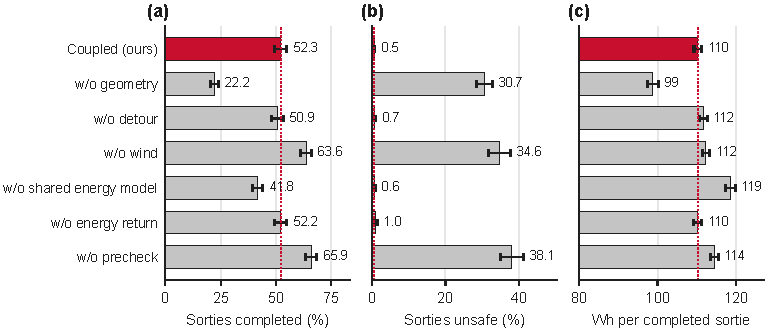
\includegraphics[width=\textwidth]{figures/pdf/ablation.pdf}
\caption{Ablation over all cities and presets (\RTLSORTIESPOL{} sorties per variant). (a) Sorties completed, (b)
sorties unsafe (lost or launched beyond the wind rating), (c) energy per completed sortie. Dotted lines mark the
coupled policy; bars show 95\% task-level bootstrap intervals}
\label{fig:ablation}
\end{figure}

\subsection{Cost of coupling}\label{sec:eval:micro}

All timings in this section come from one process pinned to one core of the server while nothing else runs; each value
is the median of seven timed calls after a warm-up, and the median over three repetitions.

\paragraph{Queries.} Batching is what makes shared models cheap (Fig.~\ref{fig:micro-queries}). A single surface-height
lookup costs 21.8\,$\mu$s, almost all of it call overhead; in batches of 10,000 it costs 0.01\,$\mu$s per point. The
corridor top along a return line, the query F1 needs, costs 63.6\,$\mu$s per line with an exact cell traversal and
0.61\,$\mu$s per line on the max-pooled height pyramid in batches of 1,000, a factor of 104. A line-of-sight test costs
9.8\,$\mu$s per pair in the maximal batch of 64. The environment field shows the same pattern: a wind query costs
27.8\,$\mu$s when issued point by point and 0.16\,$\mu$s per point in a batch of 10,000, and a slant optical depth
0.04\,$\mu$s per path. Evaluating all fields at once costs only a quarter more than wind alone, so a decision that
needs wind, visibility and density pays for one query, not three.

\begin{figure}[t]
\centering
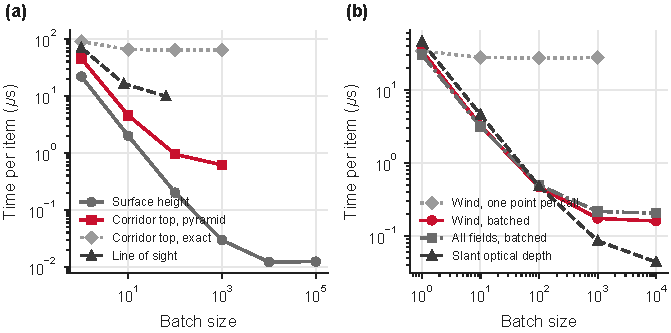
\includegraphics[width=\textwidth]{figures/pdf/micro_queries.pdf}
\caption{Query cost per item against batch size. (a) Geometry service: surface height, corridor top along a line (exact
traversal and pyramid sampling) and line of sight. (b) Environment field: wind one point per call and batched, all
fields batched, and slant optical depth}
\label{fig:micro-queries}
\end{figure}

\paragraph{Return refresh.} The rotating schedule turns the impossible schedule of F4 into a negligible one
(Fig.~\ref{fig:m4}). At 1,000 drones each 5\,Hz call refreshes 200 plans in 0.25\,ms, which amounts to 1.25
core-milliseconds per simulated second, against 3.1 for refreshing every drone at 5\,Hz, 153 for refreshing every drone
at every tick and 13,400 for doing so with exact corridors. The cost grows by a factor of 1.7 from 10 to 1,000 drones
because the fixed per-call overhead dominates; it stays below the 2 core-milliseconds the return stage is budgeted.
Plans are at most one second old, which at 3--8\,m/s is 3--8\,m of travel, well inside the 10\,m safety margin of the
clearance envelope.

\paragraph{Whole pipeline.} Figure~\ref{fig:micro-stages} runs the complete runtime with $N$ drones in rain, nearly
all flying, for 20 simulated seconds: environment, dynamics and control, sensors, contact and separation, the safety
state machines with the battery and return logic, missions and state publication, at the 4\,ms tick; scan planning and
delegation are invoked on demand and timed separately below. On a single core the runtime advances 1,000 drones at \STAGERTF{} times real time, so
real time needs \STAGECORE{} core-seconds per simulated second, inside the 0.40 budget; with 10 drones it runs
\STAGERTFTEN{} times faster than real time. Of the \STGTOT{} core-milliseconds the stages use per simulated second at
1,000 drones (\STGWALL{} including the loop around them), safety and energy take \STGSAFE{}, dynamics and control
\STGDYN{}, missions \STGMIS{}, the environment \STGENV{} and state publication \STGPUB{}. The environment stage grows
only from \STGENVTEN{} to \STGENV{} core-milliseconds between 10 and 1,000 drones, because one batched query serves
the whole fleet; the coupled decisions are thus not what limits the fleet size.

\begin{figure}[t]
\centering
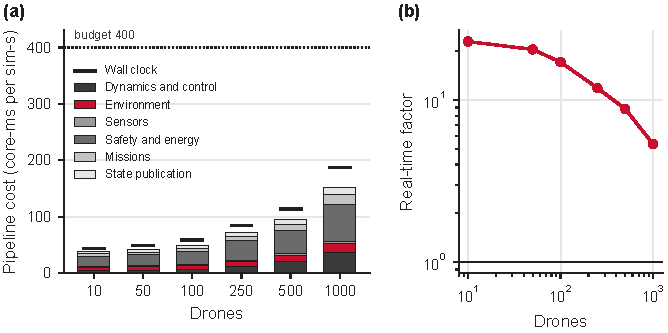
\includegraphics[width=\textwidth]{figures/pdf/micro_stages.pdf}
\caption{Whole pipeline with $N$ drones flying in rain, one core. (a) CPU cost per simulated second by stage group;
the dotted line is the 0.40 core-second budget. (b) Real-time factor (simulated seconds per wall-clock second)}
\label{fig:micro-stages}
\end{figure}

% \paragraph{Scan planner.} The perception-driven scan planner of Sect.~\ref{sec:design:decisions} plans a 0.04\,km$^2$
% area in 0.3\,s and a 4\,km$^2$ area in 2.0--2.4\,s (Fig.~\ref{fig:micro-coverage}), roughly linear in area. Planning therefore takes
% seconds, while the scans it plans take tens of minutes, and it can be rerun whenever the weather changes.

% \begin{figure}[t]
% \centering
% 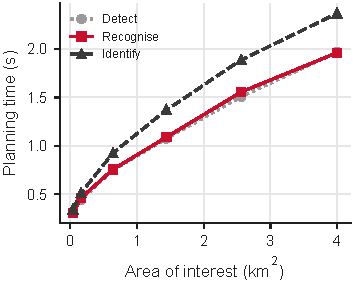
\includegraphics[width=0.55\textwidth]{figures/pdf/micro_coverage.pdf}
% \caption{Scan-planner runtime against the area of interest, per required perception level; median of three
% repetitions}
% \label{fig:micro-coverage}
% \end{figure}


\subsection{Access from ordinary devices}\label{sec:eval:access}

The server never renders; every view is drawn by the client from the streamed octree. We replay the same scripted
60\,s camera flight over Shenzhen (5.0 million points, $1600\times900$ viewport, three repetitions) on three clients:
headless Chromium with an NVIDIA A100 on the server's local network, Chrome on an Apple M3 laptop streaming from the
server over the public internet, and Chromium with the SwiftShader software renderer, a stand-in for a device
without a usable GPU. The client reports its own frame intervals, the points it draws and the screen-space error it
achieves. We compare the adaptive budget (APH with CAS) against fixed point budgets of 100k, 1M (the Potree
default~\cite{schuetz2020octree}) and 3M points (Fig.~\ref{fig:stream}).

No fixed budget is right for every device. On both GPU clients every budget reaches the display rate (16.7\,ms per
frame), and the adaptive controller raises its budget to the top of its ladder: it draws as many points as the 3M
budget and reaches the same screen-space error, below one pixel (Fig.~\ref{fig:stream}b), whereas 100k points leave a
median error of 10--14\,px. On the software renderer the picture reverses. With 1M or 3M points it renders at 12\,fps,
with a median frame time of 67--83\,ms and 83--85\% of frames beyond 1.5 times its 33.3\,ms target. The adaptive
controller holds the target (95th-percentile frame time 33.3\,ms, no frame beyond 1.5 times the target) and still draws
1.5 times as many points as the 100k budget, with a lower error (6.7 against 9.2\,px). Point selection costs at most
0.4\,ms per frame (95th percentile) on every client; slowing the M3's CPU four-fold by emulation changes neither its
frame times nor its error. The first view appears 1--2\,s after opening the page on the local network and after 14\,s
over the internet, where the 1.5\,MB first screen and the 22\,MB streamed during the flight compete with the path's
bandwidth. Because the server only serves static byte ranges and all selection runs in the client, adding viewers
adds file traffic but no per-viewer computation on the server; we did not measure many concurrent viewers.

\begin{figure}[t]
\centering
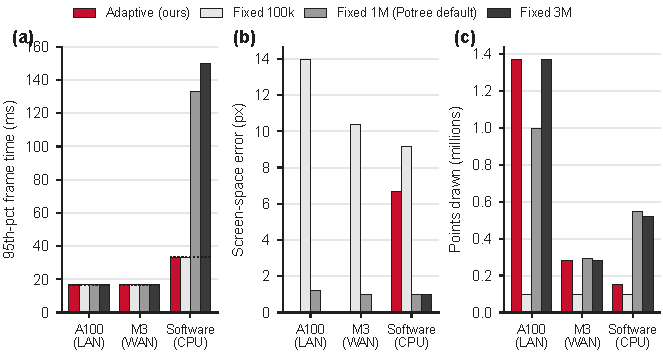
\includegraphics[width=\textwidth]{figures/pdf/stream.pdf}
\caption{The same 60\,s camera flight over Shenzhen on three clients, adaptive budget vs fixed budgets; medians of three
runs. (a) 95th-percentile frame time, with each client's frame target dotted. (b) Median screen-space error of the drawn
view. (c) Median number of points drawn}
\label{fig:stream}
\end{figure}


\subsection{Sensitivity}\label{sec:eval:sens}

Figure~\ref{fig:sens} varies the two decision parameters of the return and the visibility the scan planner faces. The
return sweeps run the coupled policy on three cities (Shenzhen, New York, SynthCity), clear weather and rain, three
seeds and all 25 combinations of the two margins; every combination flies the same sorties.

\paragraph{Clearance margin.} The margin above the corridor top trades launches for headroom
(Fig.~\ref{fig:sens}a). No setting from 0 to 20\,m lets a drone touch a building, because the clearance envelope
already contains a 10\,m safety margin and a 4\,m dilation. Larger margins raise the cruise and return altitudes,
which costs energy: at 20\,m the precheck declines 38.2\% of sorties instead of 27.1\% at the default of 5\,m, and
completion falls from 59.0\% to 50.7\%. Below 5\,m the gain is at most 1.4 points. The only contact in the sweep at a
margin of 0\,m is between two drones whose transit and return paths then coincide; inter-drone separation is handled by
the runtime's separation guard, not by the return planner.

\paragraph{Trigger margin.} The return starts when the remaining flight time falls below a multiple of the
energy-equivalent return time. Between 1.0 and 1.5 the outcome does not change (Fig.~\ref{fig:sens}b): with the shared
energy model the trigger is rarely the binding constraint, because the precheck has already budgeted the return. At 1.8
it recalls 16.7\% of sorties early instead of 13.9\% and completes 4.2 points fewer. The default of 1.3 sits in the flat
region, so the result does not depend on tuning it.

\paragraph{Visibility.} The coupled scan planner keeps capture within a few points of the clear-air ceiling down to a
MOR of about 200\,m (Fig.~\ref{fig:sens}c), where the weather-blind plan has already lost almost every target
(Fig.~\ref{fig:m3}a). It pays with drones: a recognition scan needs 1.76 drones on average in clear air, 2.29 at
200\,m and 3.19 at 100\,m. At 100\,m capture drops to 51--74\%, and 19--43\% of the plans are declined because no
lens resolves the target from a height that clears the buildings; the planner reports this before launch. The wind
sweep of Fig.~\ref{fig:m2} gives the corresponding sensitivity of launch and return to wind speed.

\begin{figure}[t]
\centering
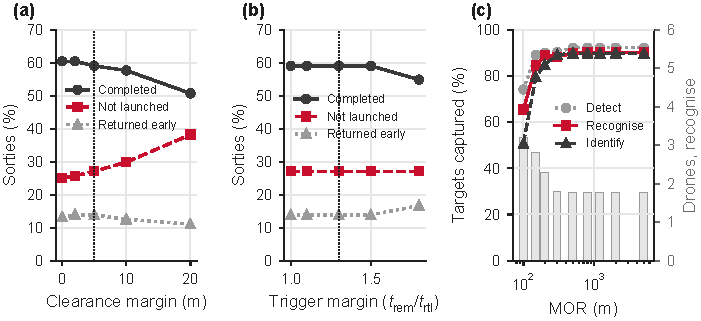
\includegraphics[width=\textwidth]{figures/pdf/sensitivity.pdf}
\caption{Sensitivity of the coupled policy. (a) Clearance margin above the corridor top and (b) return-trigger margin,
on the same 216 sorties per setting in clear weather and rain; dotted lines mark the defaults. (c) Scan planning under
a MOR sweep: targets captured at each level (lines, left axis) and drones a recognition scan needs (bars, right axis)}
\label{fig:sens}
\end{figure}


\subsection{Consistency and reproducibility}\label{sec:eval:consistency}

The design promises one model evaluated identically by the planner, the runtime and the display, and runs that are a
deterministic function of their seed. Table~\ref{tab:consistency} tests both. For the environment field we evaluate the
browser implementation on the golden vectors produced by the server implementation, over every function the display
uses. Of 79,104 outputs, 98.7\% are bit-identical and the largest absolute difference is $3.6\times10^{-12}$, from
floating-point reassociation in the wind composition; these differences are about ten orders of magnitude below the resolution of any decision threshold
(centimetres, tenths of a metre per second) and below single-precision rendering. For the fleet
runtime we run 18 configurations (three cities, clear, fog and thunderstorm weather, two seeds) three times each in
separate processes, with 16 drones flying for 180\,s in gusty wind, and hash the full fleet state every simulated
second. All 3,240 checkpoints agree across the three runs.

% generated by paper/figures/gen_numbers.py
\begin{table}[t]
\caption{Consistency of the shared environment model between the server and the browser, and replay determinism of the fleet runtime.}\label{tab:consistency}
\footnotesize
\begin{tabular*}{\textwidth}{@{\extracolsep{\fill}}lrrr@{}}
\toprule
Environment function & Outputs & Bit-identical & Max.\ abs.\ difference \\
\midrule
Field evaluation (wind, gust, optics) & 28,350 & 99.5\% & $3.6\times10^{-12}$ \\
Derived weather quantities & 19,228 & 99.9\% & $1.8\times10^{-15}$ \\
Wind sectors and slots & 17,352 & 100.0\% & 0 \\
Frame and unit conventions & 10,324 & 91.7\% & $5.7\times10^{-14}$ \\
Gust events & 1,837 & 99.9\% & $2.8\times10^{-16}$ \\
Slant optical depth & 687 & 93.4\% & $7.1\times10^{-15}$ \\
Turbulence box & 612 & 100.0\% & 0 \\
Standard atmosphere & 360 & 100.0\% & 0 \\
Keyframe anchors & 252 & 99.2\% & $6.7\times10^{-16}$ \\
Vertical wind profile & 102 & 100.0\% & 0 \\
\emph{All environment functions} & 79,104 & 98.7\% & $3.6\times10^{-12}$ \\
\midrule
Fleet replay (state hash per second) & 3,240 & 100\% & 0 \\
\bottomrule
\end{tabular*}
\end{table}


% \section{Discussion and limitations}\label{sec:discussion}

\paragraph{Reference models.} The energy, wind and perception models are reference models: a P600-class hexacopter
power model, an analytic urban wind and visibility field driven by twelve weather presets, and the Johnson criteria with
Koschmieder contrast attenuation. We report relative differences between policies on the same ground truth because
these differences depend on the coupling, not on the calibration of one vehicle. Absolute endurance, wind loads near
buildings and detection probabilities of a specific drone and camera will differ, and calibrating the models against
flight logs, measured urban wind and camera imagery is the next step. Because every model sits behind one interface,
a calibrated model replaces the reference one for all modules at once, which is the point of sharing it.

\paragraph{Geometry.} Safety is certified against the city's surface model at 2\,m resolution, dilated by 4\,m and
raised by a 10\,m margin. Wires, cranes, thin structures, overhangs and changes after the point cloud was captured are
not in the model, and the margin is not a substitute for onboard sensing. The runtime treats the surface model as one
input to the decision and the separation and contact stages as another; an onboard obstacle-avoidance layer remains
necessary in real operations.

\paragraph{Weather in time.} The environment field represents a forecast as a keyframe transition, and the space-time
precheck uses it as if it were exact. Real forecasts are uncertain in timing and strength; a precheck that plans
against an ensemble of transitions, and a return trigger that re-plans when the forecast changes in flight, are natural
extensions. The precheck also samples the route wind at a few points per leg, which left 4--11\% of sorties meeting
wind beyond the rating on the path they actually flew.

\paragraph{Scope of the evaluation.} Scan plans are scored on their planned trajectories with the perception model
rather than flown in closed loop, and the closed-loop campaigns use eight drones per task; the 1,000-drone measurements
show that the runtime keeps the coupled return logic inside the real-time budget, not that decisions remain equally
good when hundreds of drones interact. Browser access was measured on a laptop, a software renderer and a data-centre
GPU, and the server's cost per additional viewer was not measured. These are limits of the present evaluation, not of
the design, and the open-source release includes the harness to extend it.

\paragraph{Safety and dual use.} The runtime is a planning and simulation tool for civil fleet operations. It does not
replace airworthiness assessment, airspace authorisation or onboard safety functions, and its outputs should be used
with the margins that local regulations require.

\section{Conclusion}\label{sec:conclusion}

Urban drone decisions depend on the city, the weather and the battery at once, and a decision that sees only part of
this picture fails in systematic, city- and weather-dependent ways: returns fly into buildings, modules contradict each
other in wind, and scans miss their targets without noticing. We presented Drone4D, a space-time world runtime that serves one model of
geometry, weather and energy to the planner, the fleet runtime and the browser, and a decision layer that couples the
launch precheck, return planning, scan planning and task delegation to it. Batched queries on one clock and a rotating
refresh make the coupling cheap enough for 1,000 drones on one CPU core. In closed-loop campaigns over seven cities and
twelve weather conditions, coupling reduced unsafe sorties from \PXUNSAFE\% to \CPUNSAFE\% while doubling the share of
completed sorties, kept sorties out of a forecast weather front, restored recognition capture in fog and raised the
success of task delegation. Each coupling removes a different failure, and none of them alone delivers both safety and
productivity. 
The runtime, the experiment harness, the raw results and the figure scripts are released as open source,
so that calibrated vehicle, weather and perception models can be plugged into the same shared interfaces.


\backmatter

\section*{Statements and Declarations}

\begin{itemize}
% \item \textbf{Funding.} [Funding information to be added by the authors.]
\item \textbf{Competing interests.} The authors have no competing interests to declare that are relevant to the
content of this article.
\item \textbf{Ethics approval and consent to participate.} Not applicable. The study involves no human participants,
human data or animals; all experiments are simulations.
\item \textbf{Consent for publication.} Not applicable.
\item \textbf{Data availability.} The raw results of every experiment (one table per campaign) and the scripts that
produce every figure and number in this article are available in the \texttt{paper/} directory of the project
repository, \url{https://github.com/ANetResearch/ANet-Drone4D}. The city point clouds are derived from the public
UrbanScene3D dataset~\cite{lin2022urbanscene3d}.
\item \textbf{Code availability.} The runtime, the decision layer and the experiment harness are open source at
\url{https://github.com/ANetResearch/ANet-Drone4D}; \texttt{tools/paper/} contains the experiment harness and
\texttt{paper/figures/} the figure scripts; \texttt{paper/README.md} lists the command that produced each data set.
% \item \textbf{Author contributions.} Conceptualization: Miaohui Song, Mu Yuan, Jinke Song; Methodology: Miaohui Song,
% Jinke Song; Software: Miaohui Song, Mu Yuan; Investigation and formal analysis: Miaohui Song, Mu Yuan, Shengyuan Ye;
% Writing -- original draft preparation: Miaohui Song; Writing -- review and editing: Mu Yuan, Jinke Song, Shengyuan Ye,
% Lan Zhang; Resources: Jinke Song; Supervision: Jinke Song, Lan Zhang. All authors read and approved the final
% manuscript.
% \item \textbf{Use of large language models.} Large language models were used to help search the literature (every
% reference was checked against its publisher or arXiv record), to assist with drafting and editing the text, and to
% produce a simulated reviewer critique of the draft (Sect.~\ref{sec:eval:setup}). All experiments, data and figures were
% produced by code in the project repository, and the authors take full responsibility for the content.
\end{itemize}

\bibliography{refs}

\end{document}
